\chapter{Results}
\label{chapter:results}

\section{How to add images}

A simple image can be added like this.

\begin{figure}[!htb]
	\centering
	
	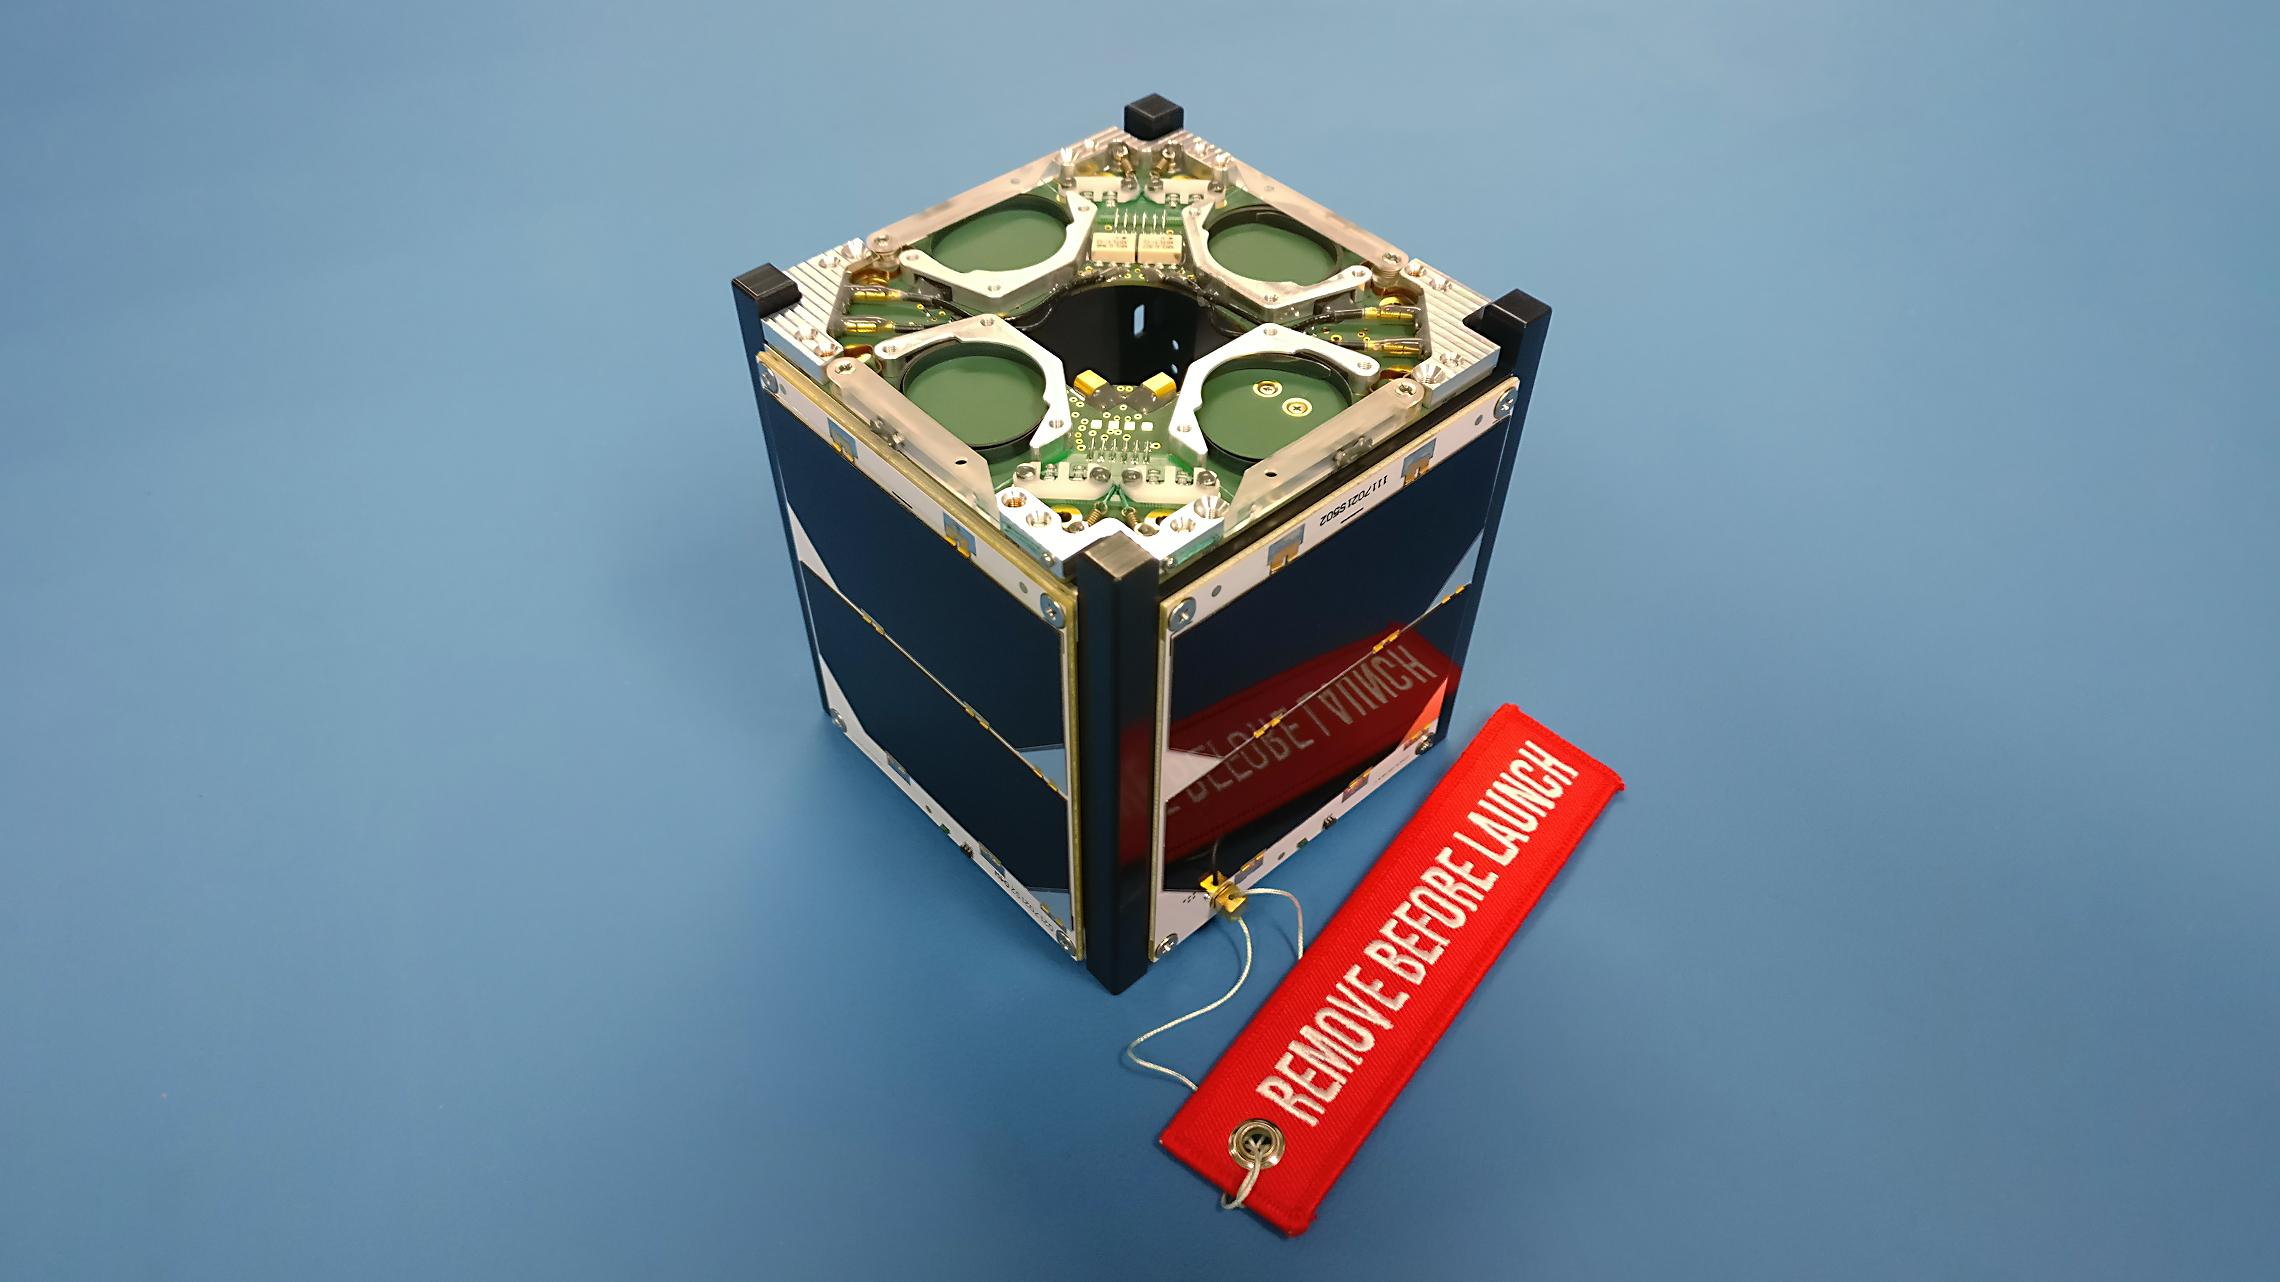
\includegraphics[width=.5\textwidth]{images/istsat1.jpeg}
	\caption[This piece of text is the image caption that will be shown in the list of tables at the start of the document.]{This piece of text will show up under the image itself. Having 2 different captions is useful when you want a long caption to appear next to the image itself since (as you can imagine) it won't look great to have a big description for a single figure in the list of figures.}
	\label{fig:normal_image}
\end{figure}

Figure \ref{fig:normal_image} shows a picture of ISTSat-1, a 1U CubeSat developed at Técnico. You can learn more about ISTSat-1 on \href{https://110.tecnico.ulisboa.pt/arquivos/episodio-34-istsat-1-o-1-o-cubesat-portugues/}{this} episode of the ``110 Histórias, 110 Objetos'' podcast or on the project's website: \url{https://istsat.one}.

What if you need something more difficult than just a single image? What if you need 2 images side by side? 

You can use the example code for Figure \ref{fig:subfigure_env} to have subcaptions for each of your subfigures and then a caption for both images.

%%%%%%%%%%%%%%%%%%%%%%%%% SUBFIGURE %%%%%%%%%%%%%%%%%%%%%%%%%
\begin{figure}[!htb]
    \centering
    \begin{subfigure}{.4\textwidth}
        \centering
        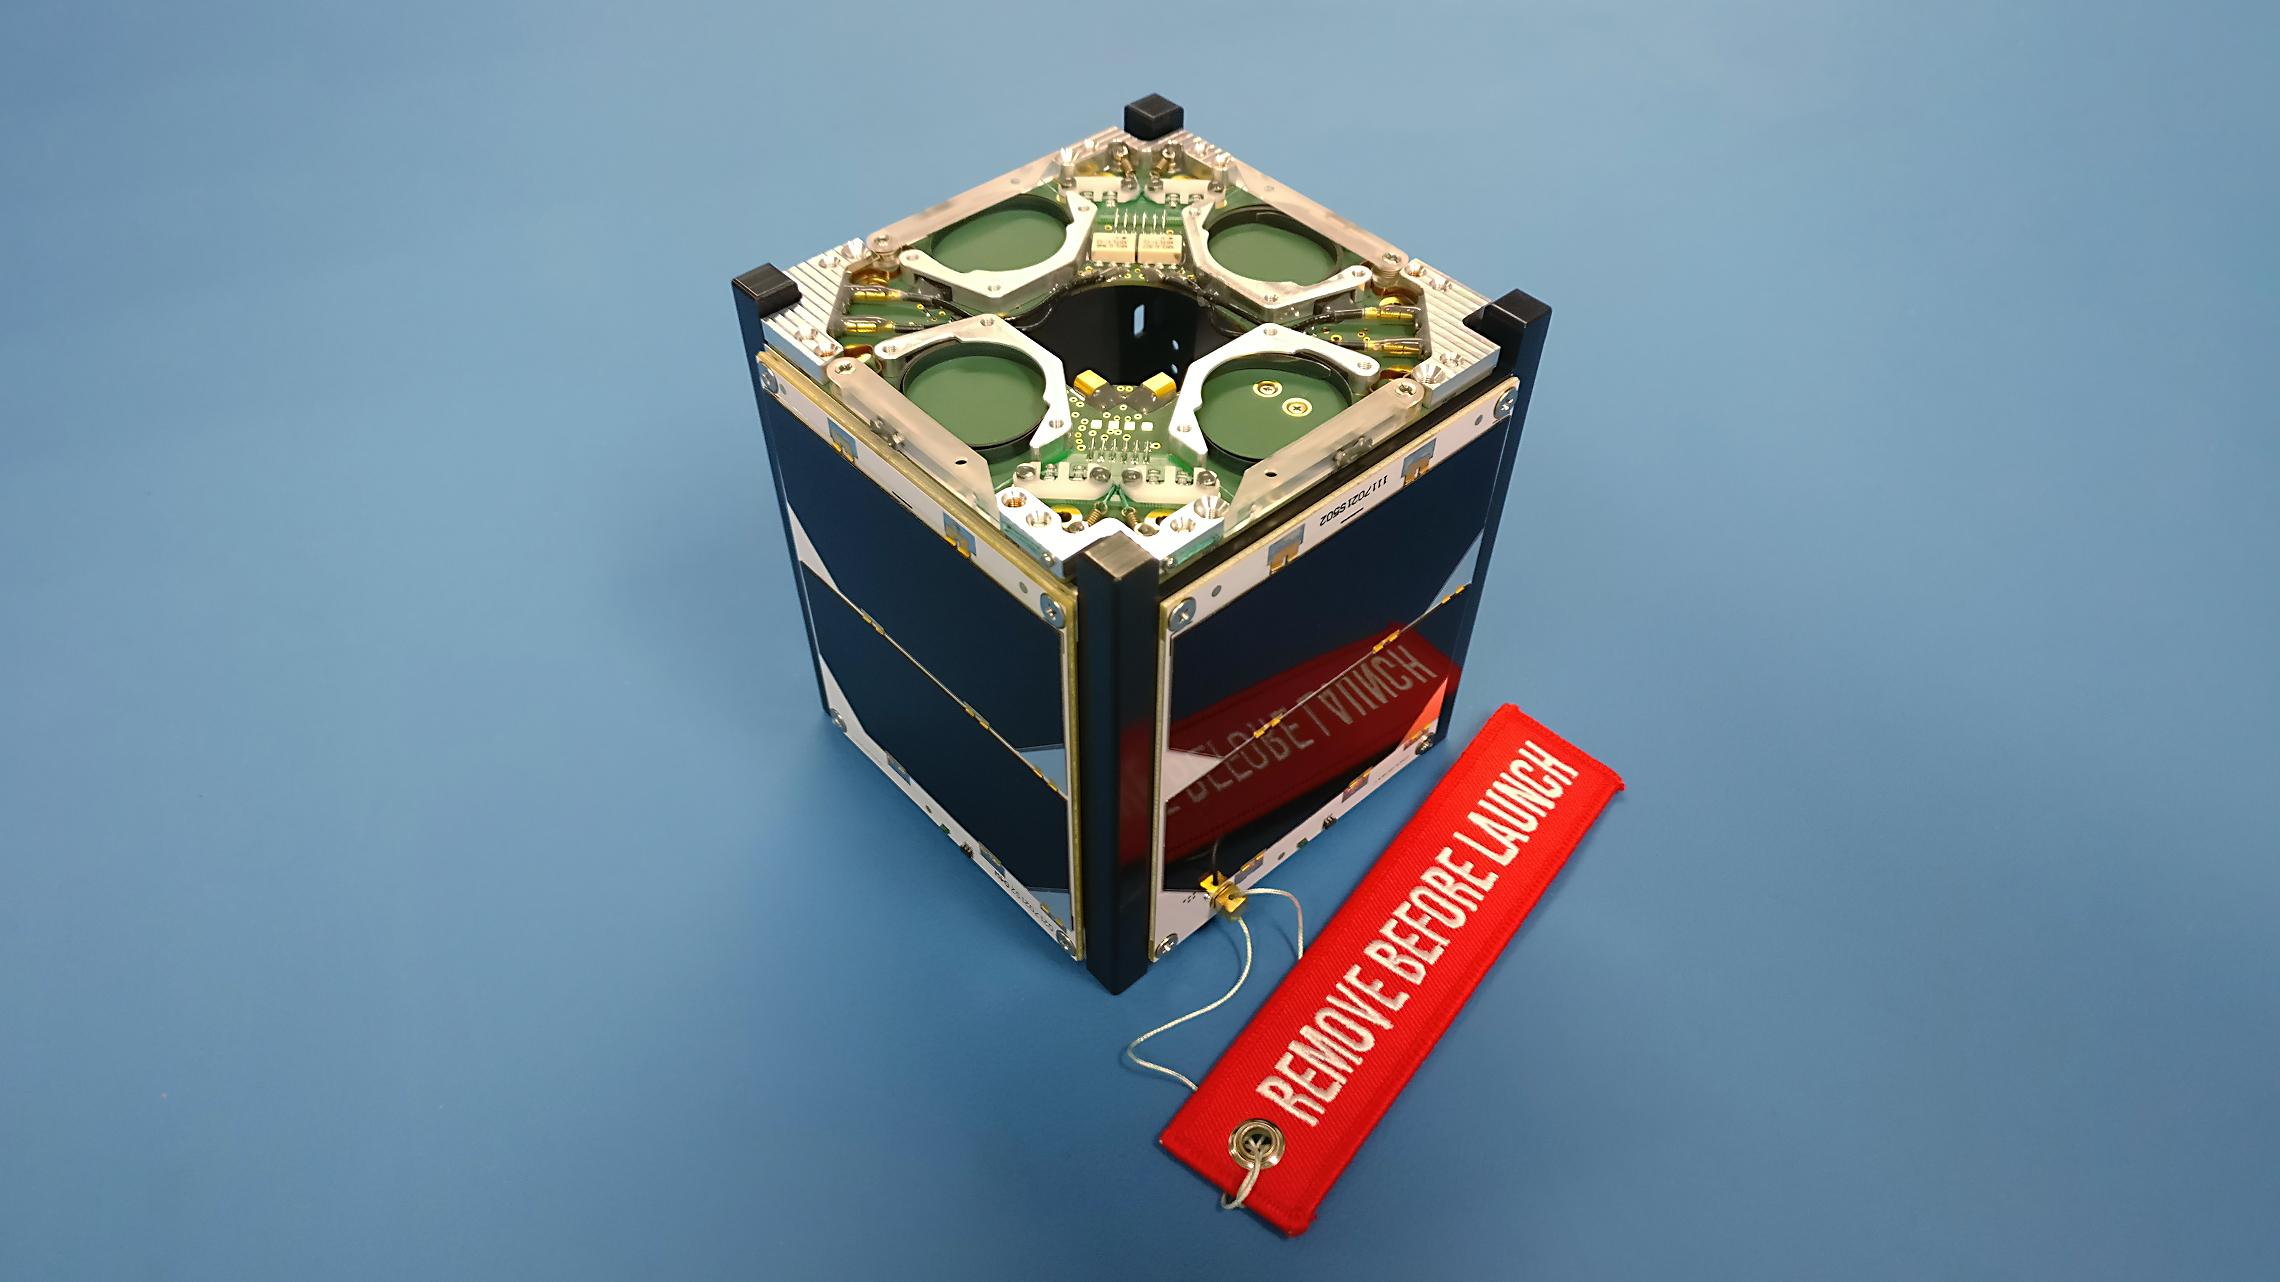
\includegraphics[width=\textwidth]{images/istsat1.jpeg}
        \caption{A caption.}
    \end{subfigure}
    \hfill
    \begin{subfigure}{.4\textwidth}
        \centering
        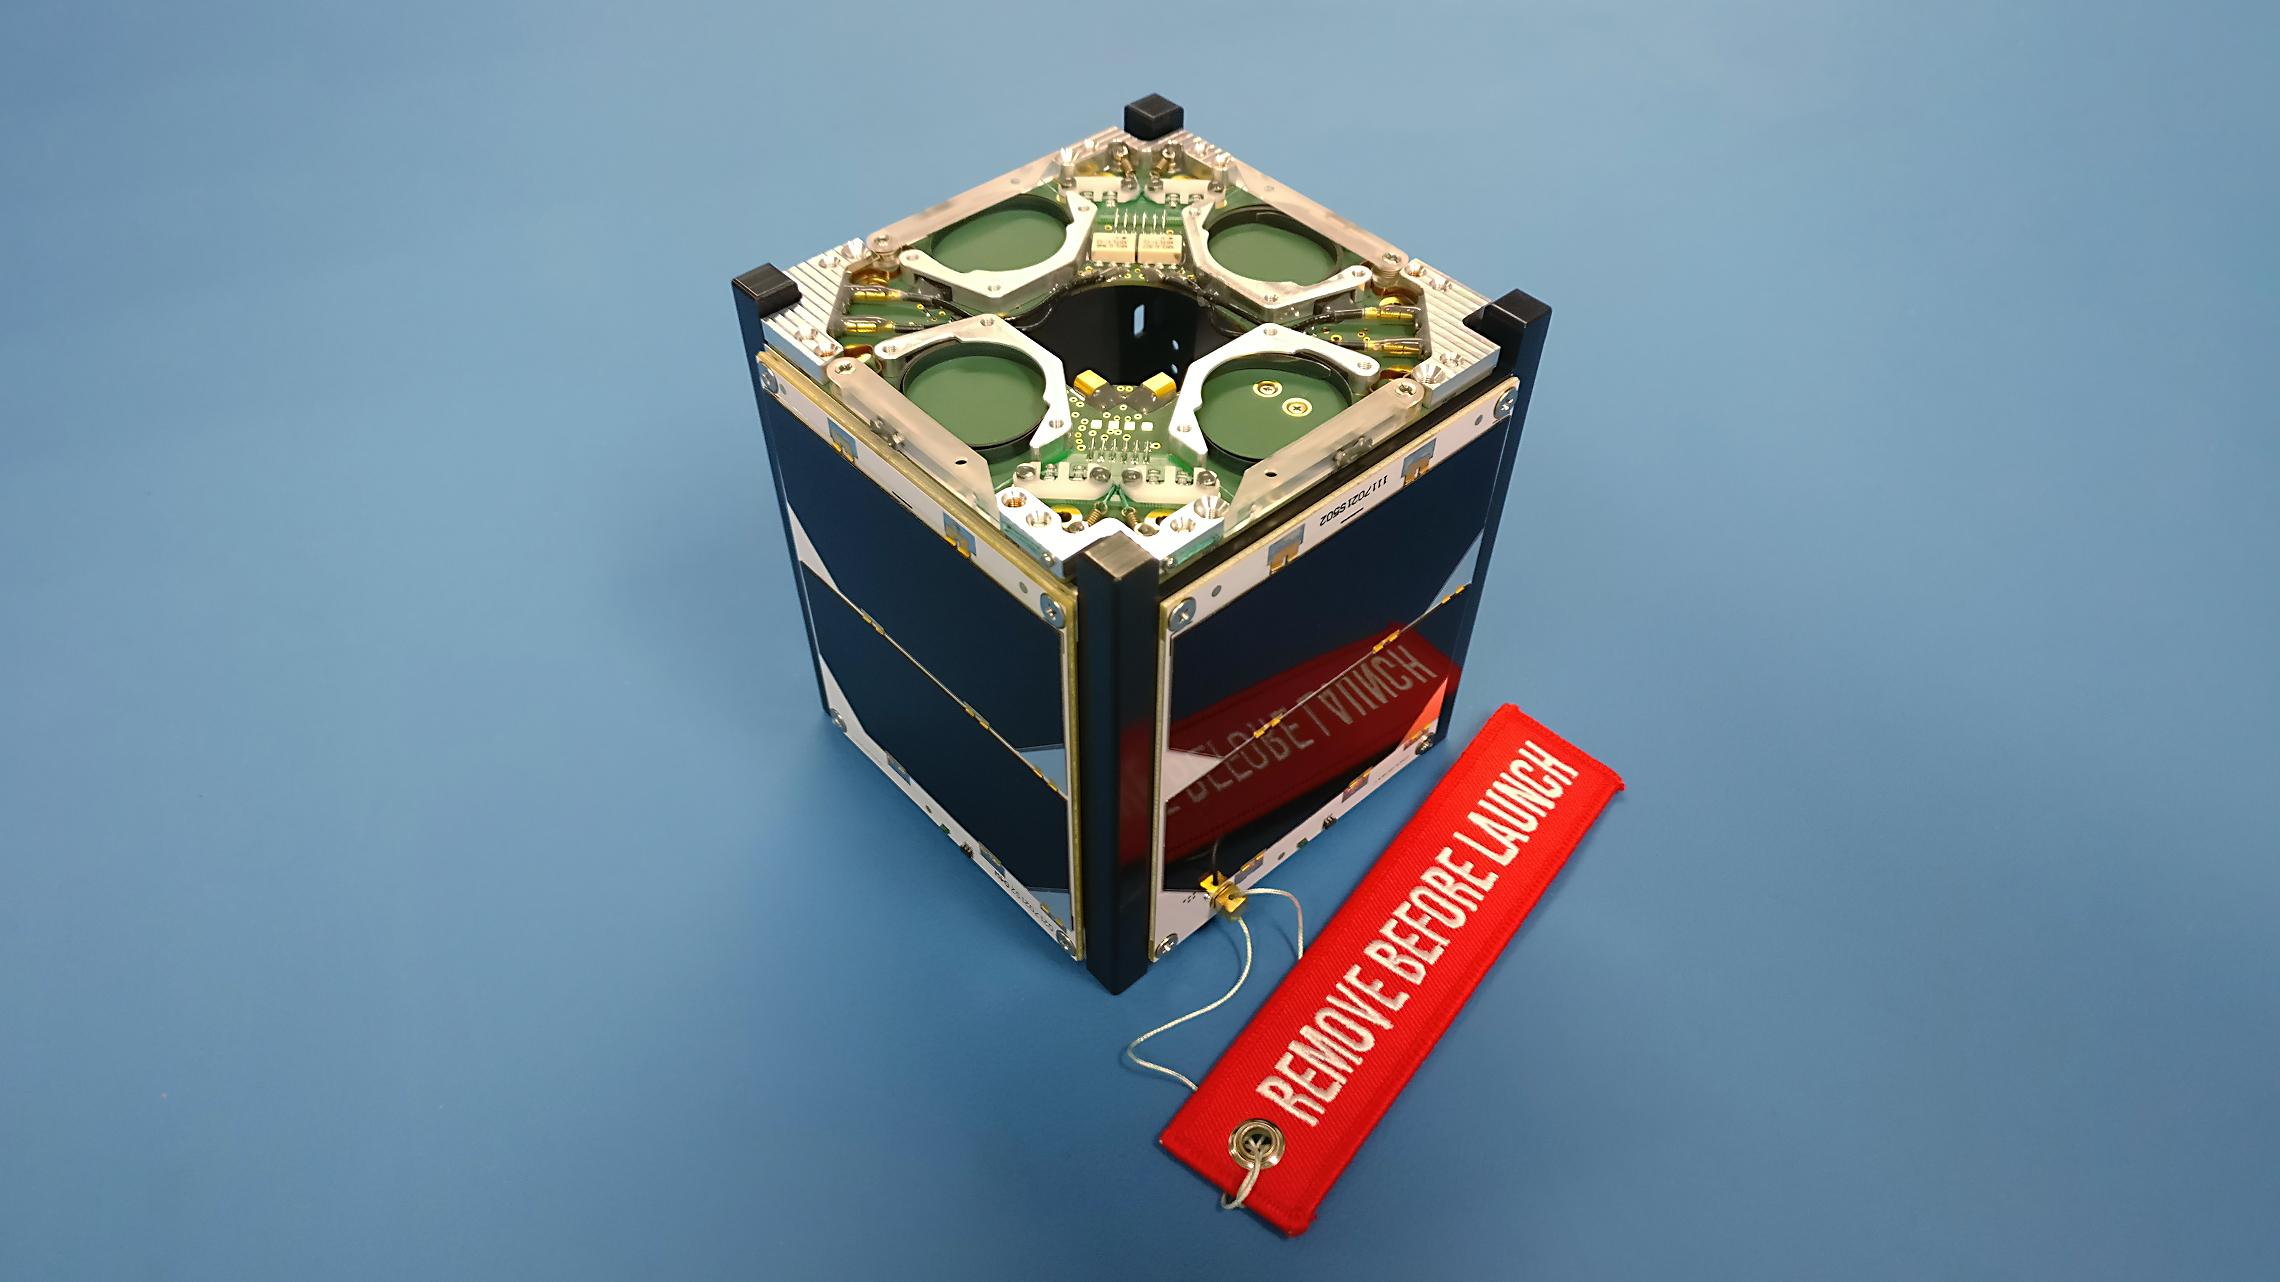
\includegraphics[width=\textwidth]{images/istsat1.jpeg}
        \caption{Another caption.}
    \end{subfigure}
    \caption{This example uses the subfigure environment. You can play with the space between images and image size by changing the percentages that are multiplied by ``textwidth'' for the images' widths.}
	\label{fig:subfigure_env}
\end{figure}

However, if yiu just want to have 2 completely independent images side-by-side, just use the example code for Figures \ref{fig:minipage_env_1} and \ref{fig:minipage_env_2}.

%%%%%%%%%%%%%%%%%%%%%%%%% MINIPAGE %%%%%%%%%%%%%%%%%%%%%%%%%
\begin{figure}[!htb]
    \centering
    \begin{minipage}{.45\linewidth}
        \centering
        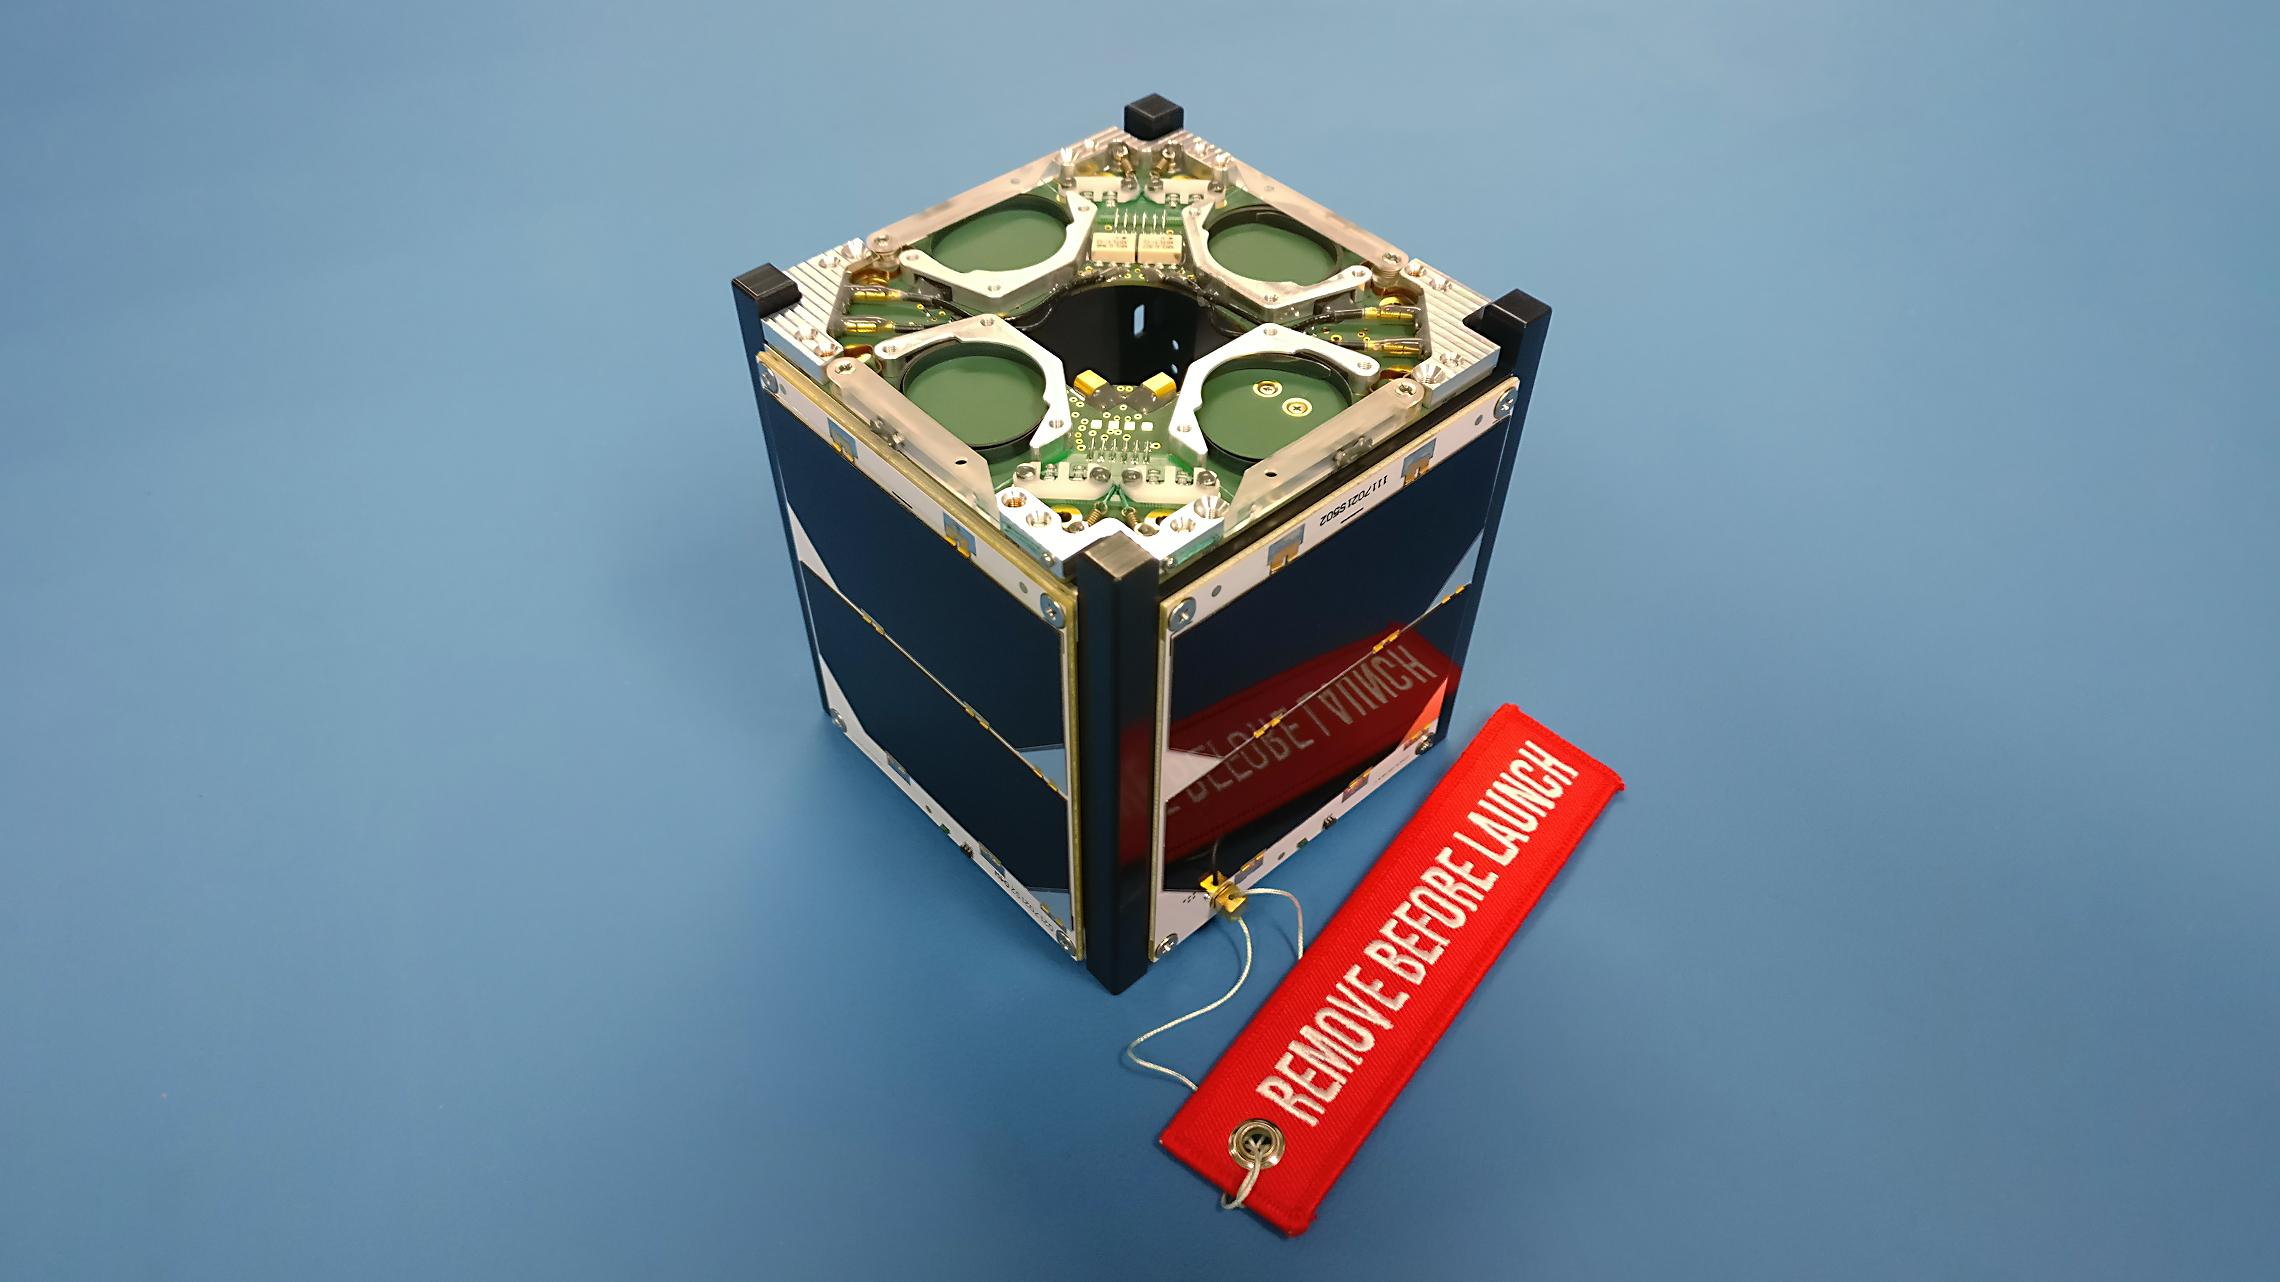
\includegraphics[width=0.6\textwidth]{images/istsat1.jpeg}
        \caption{An independent caption.}
		\label{fig:minipage_env_1}
    \end{minipage}
    \begin{minipage}{.45\linewidth}
        \centering
        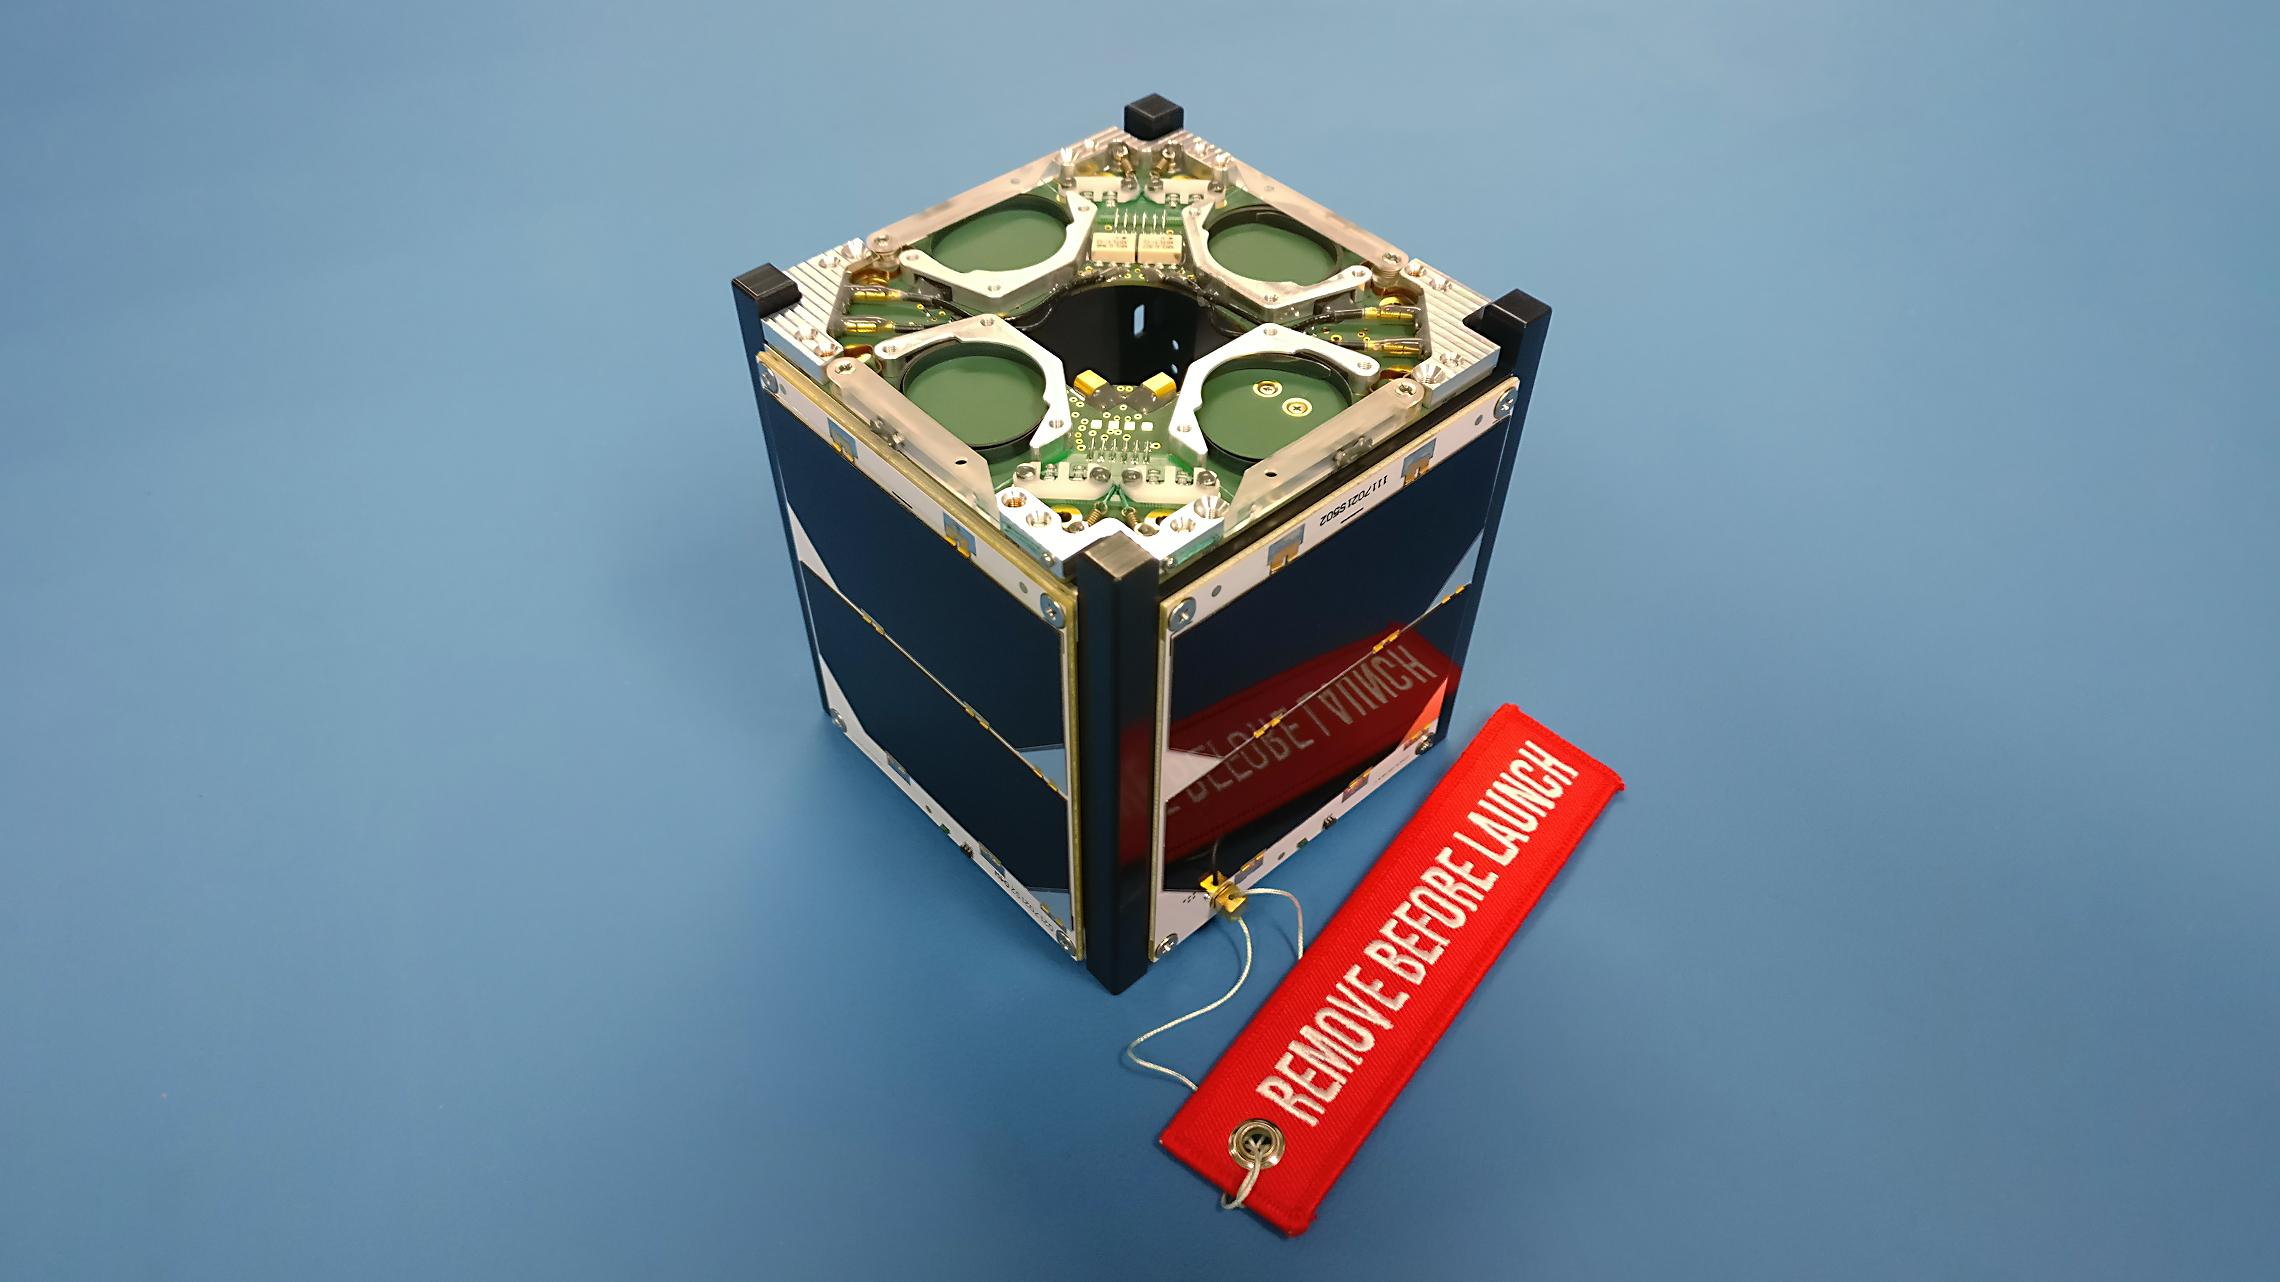
\includegraphics[width=0.6\textwidth]{images/istsat1.jpeg}
        \caption{Another independent caption.}
		\label{fig:minipage_env_2}
    \end{minipage}
\end{figure}

What if you need more than 2 images side by side? Follow the example of Figures \ref{fig:four_in_row_1}, \ref{fig:four_in_row_2}, \ref{fig:four_in_row_3} and \ref{fig:four_in_row_4}.

\begin{figure}[!htb]
    \centering
    \begin{minipage}{.2\linewidth}
        \centering
        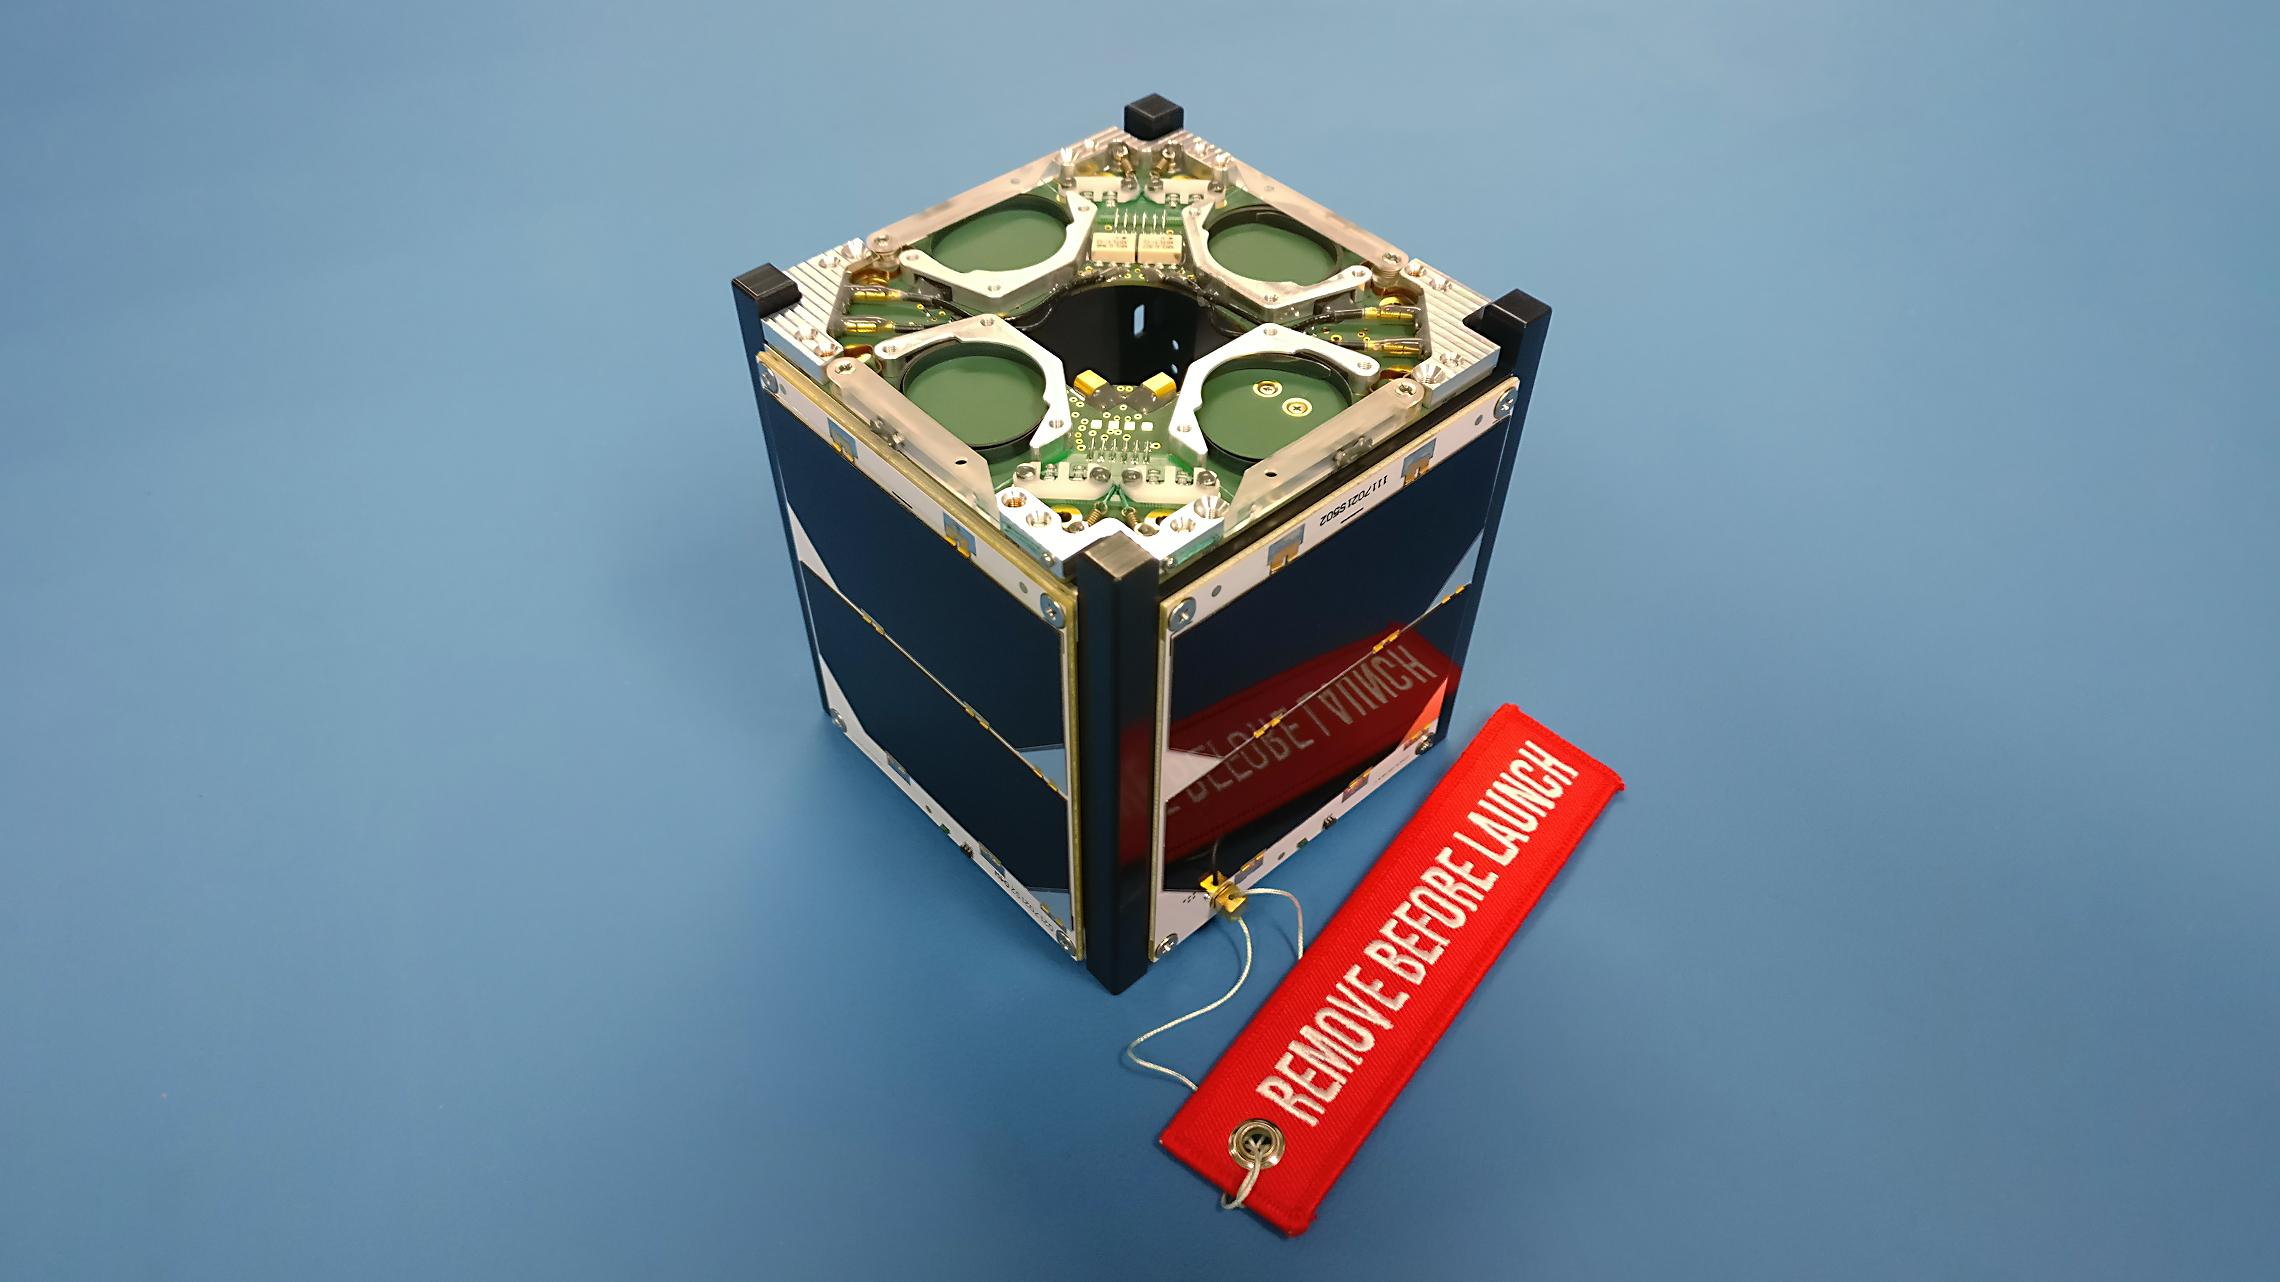
\includegraphics[width=0.95\textwidth]{images/istsat1.jpeg}
        \caption{An independent caption.}
		\label{fig:four_in_row_1}
    \end{minipage}
    \begin{minipage}{.2\linewidth}
        \centering
        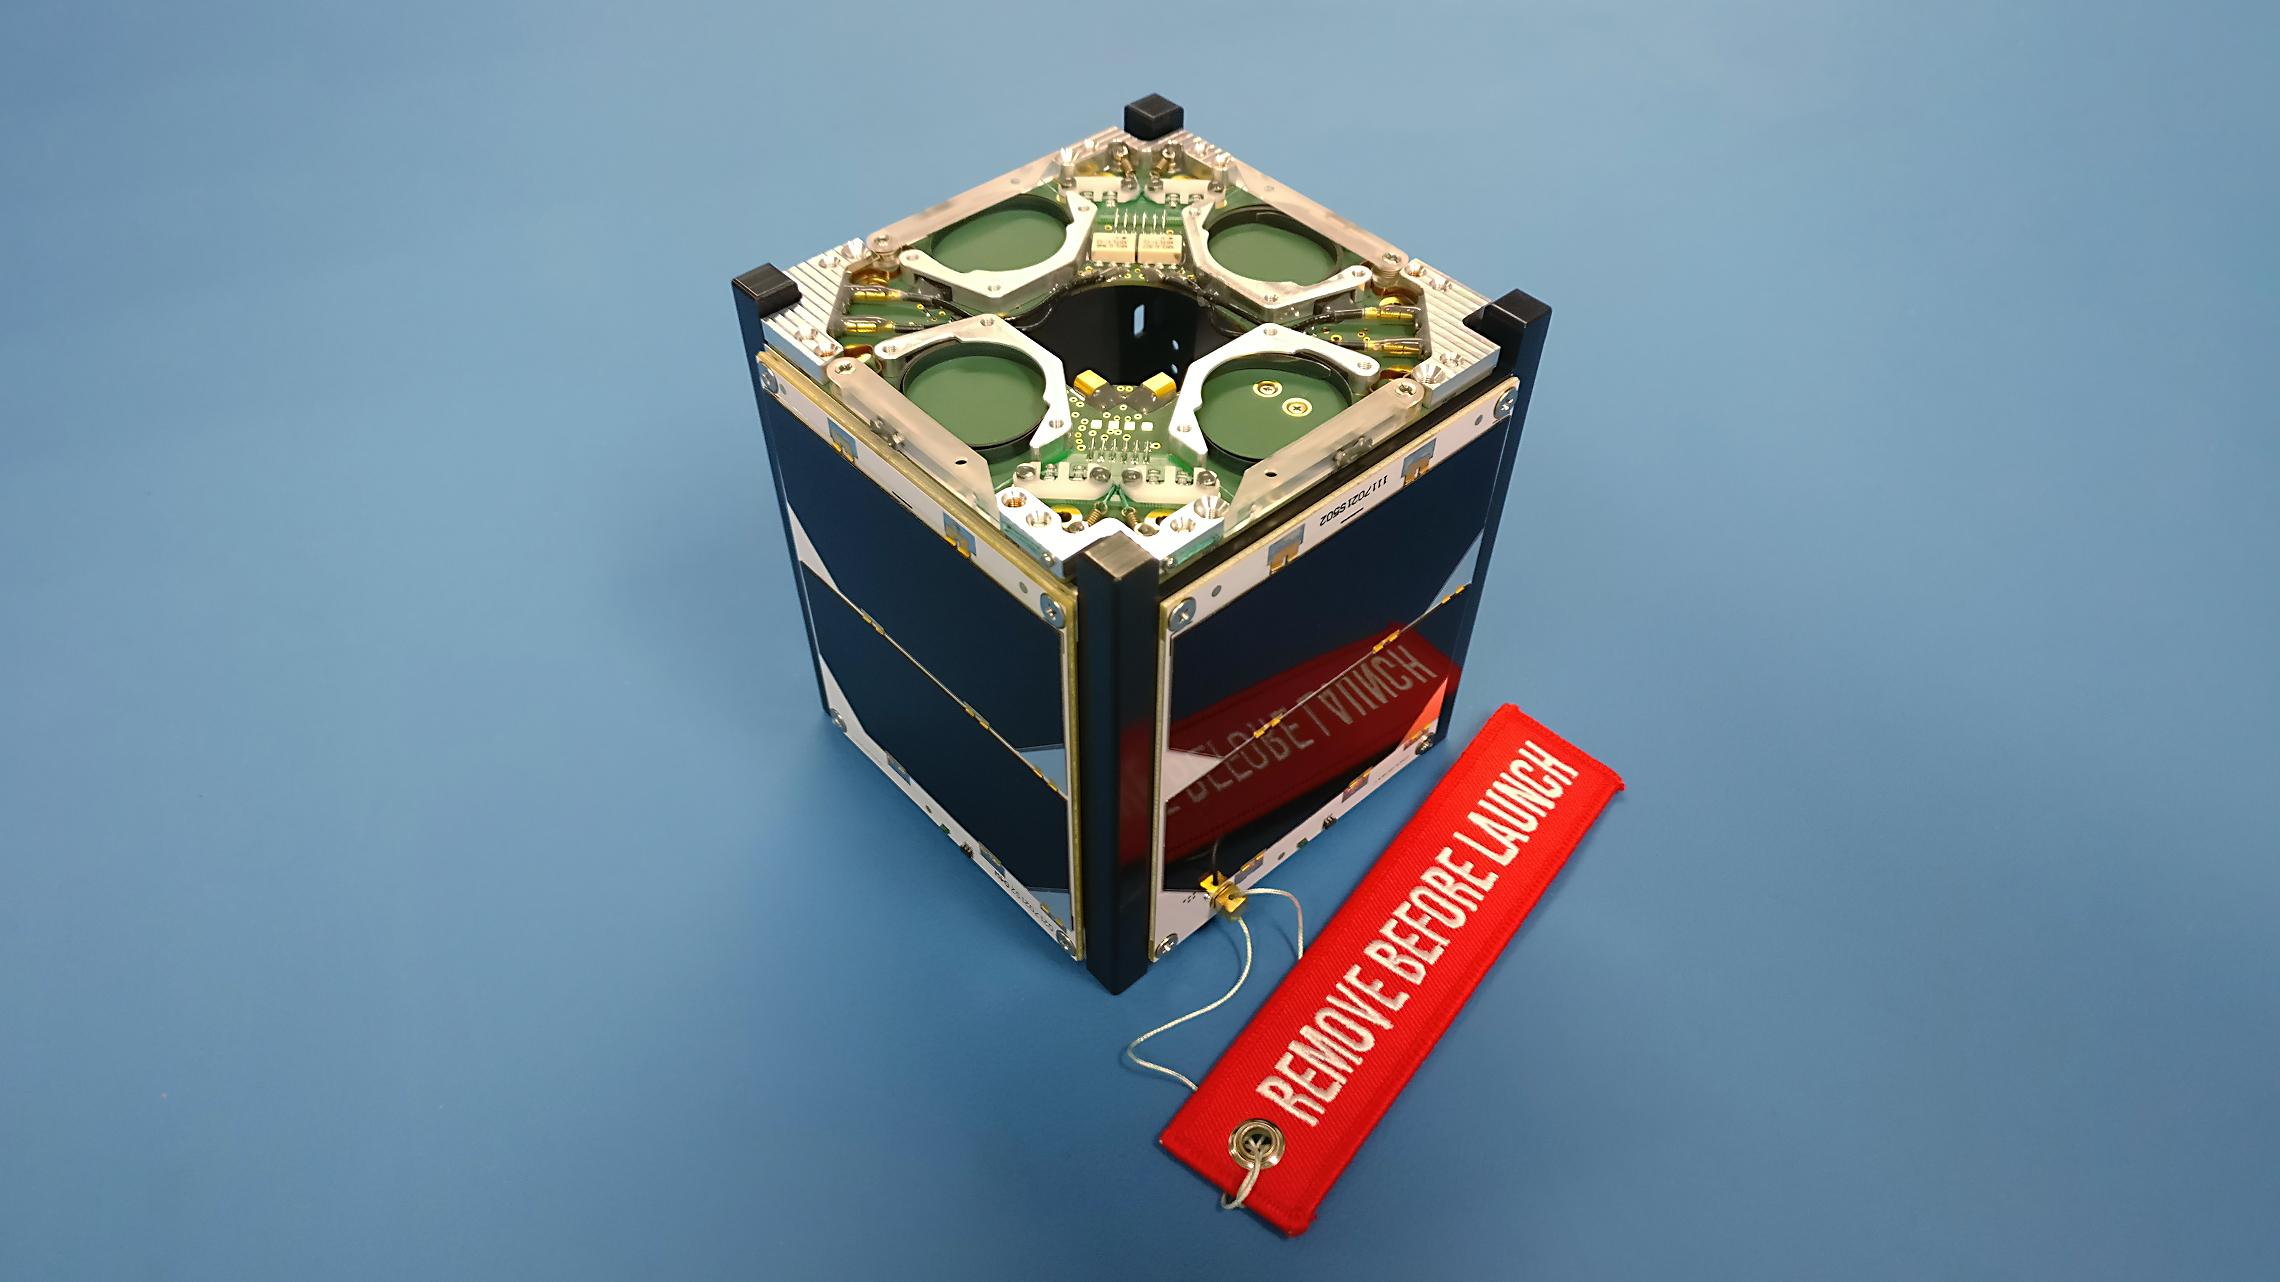
\includegraphics[width=0.95\textwidth]{images/istsat1.jpeg}
        \caption{Another independent caption.}
		\label{fig:four_in_row_2}
    \end{minipage}
	\begin{minipage}{.2\linewidth}
        \centering
        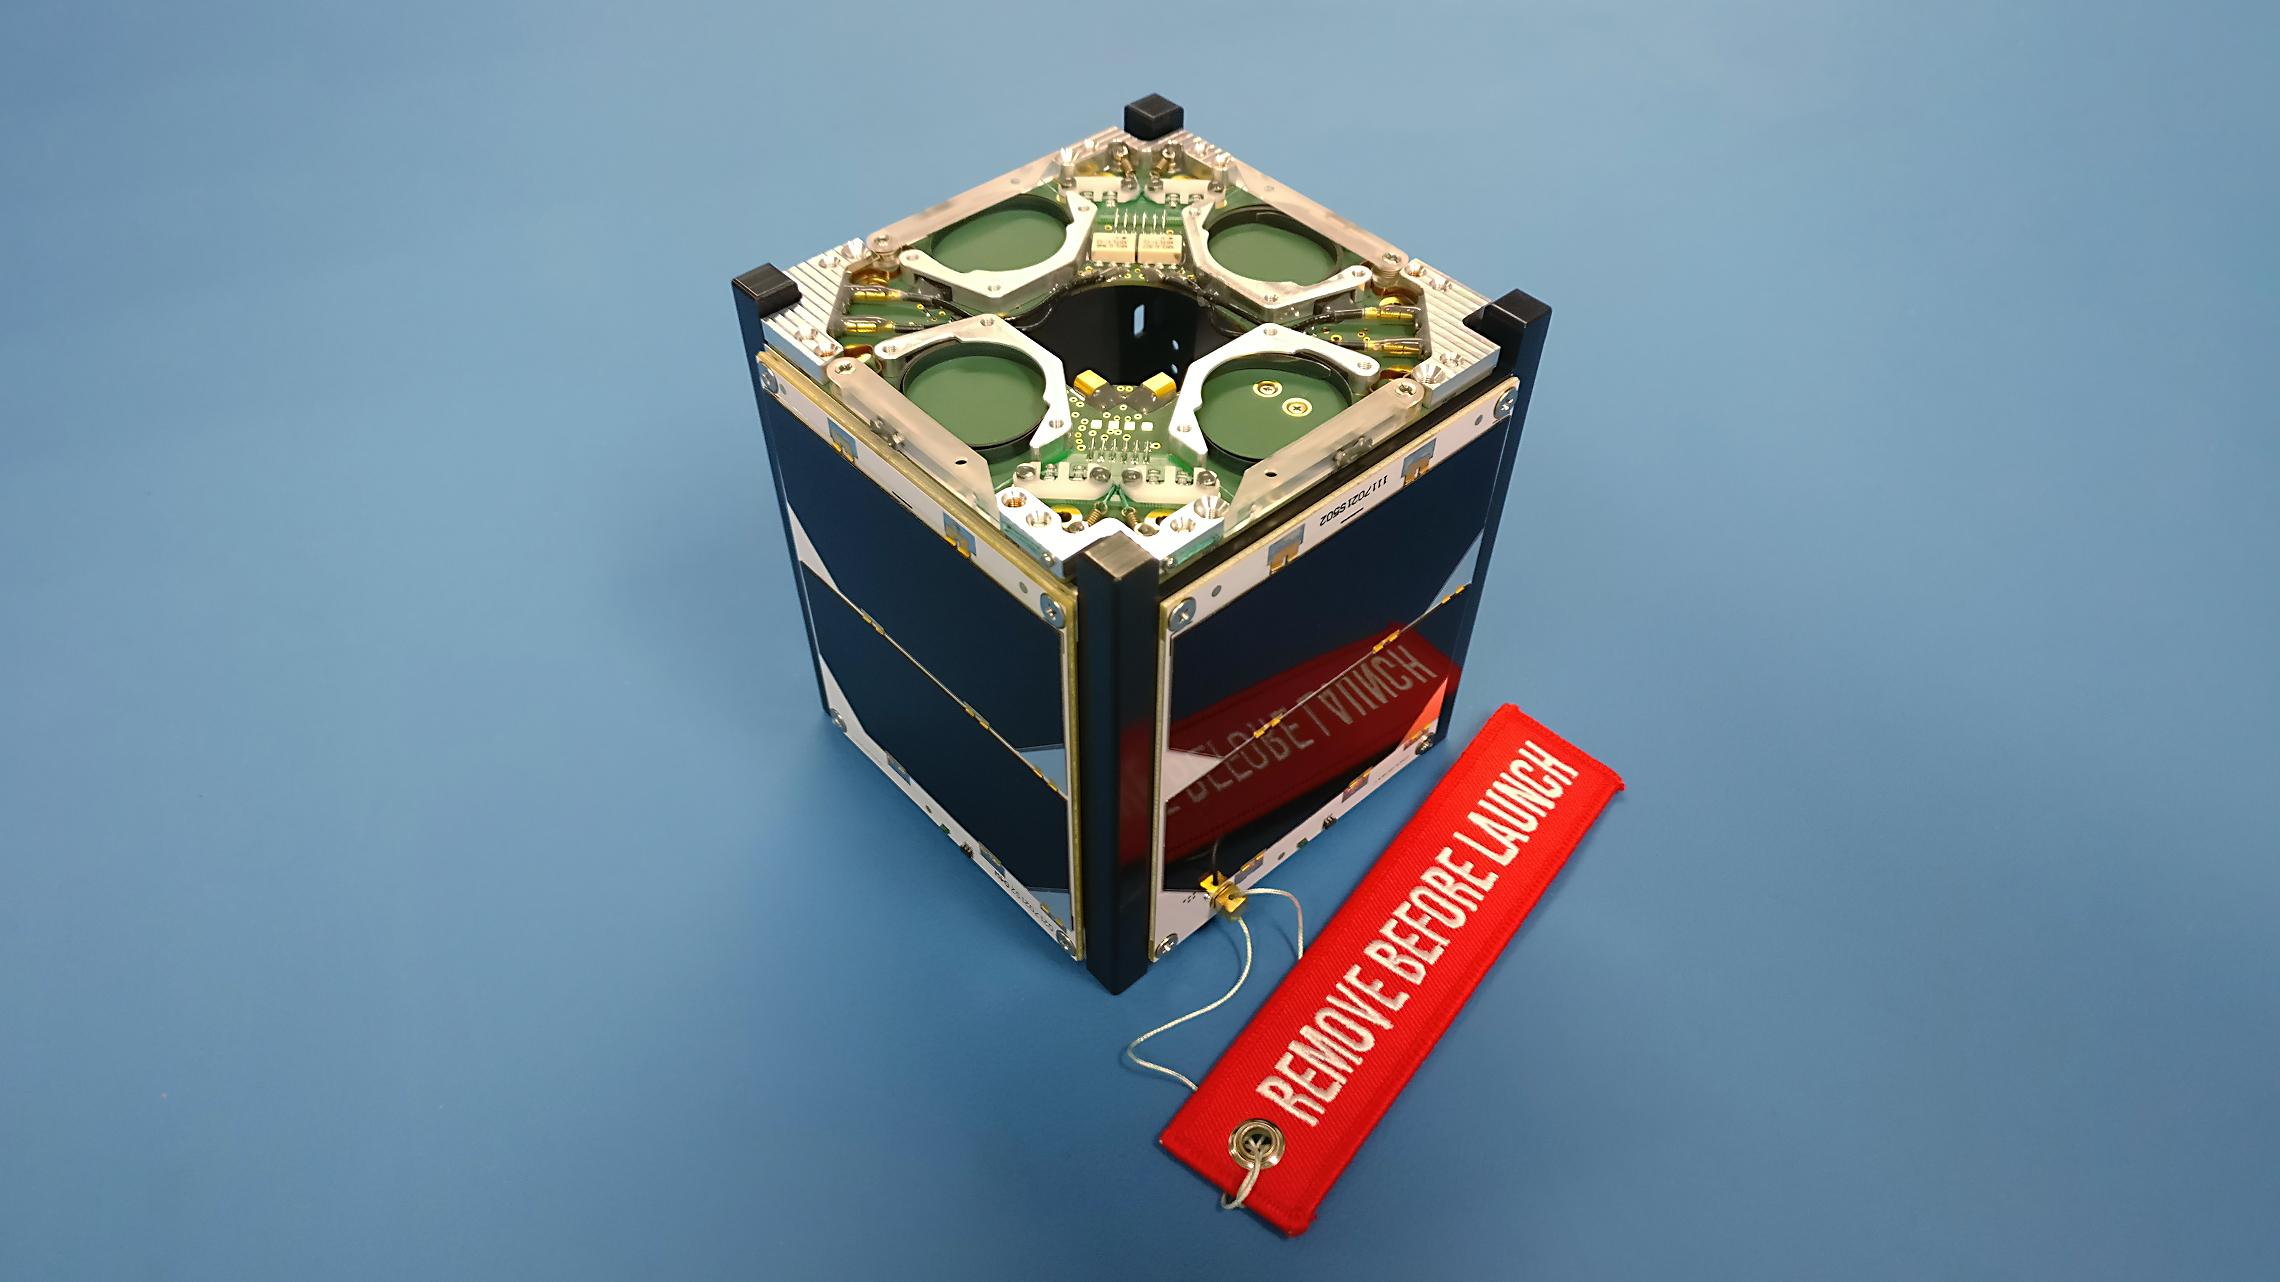
\includegraphics[width=0.95\textwidth]{images/istsat1.jpeg}
        \caption{Another independent caption.}
		\label{fig:four_in_row_3}
    \end{minipage}
	\begin{minipage}{.2\linewidth}
        \centering
        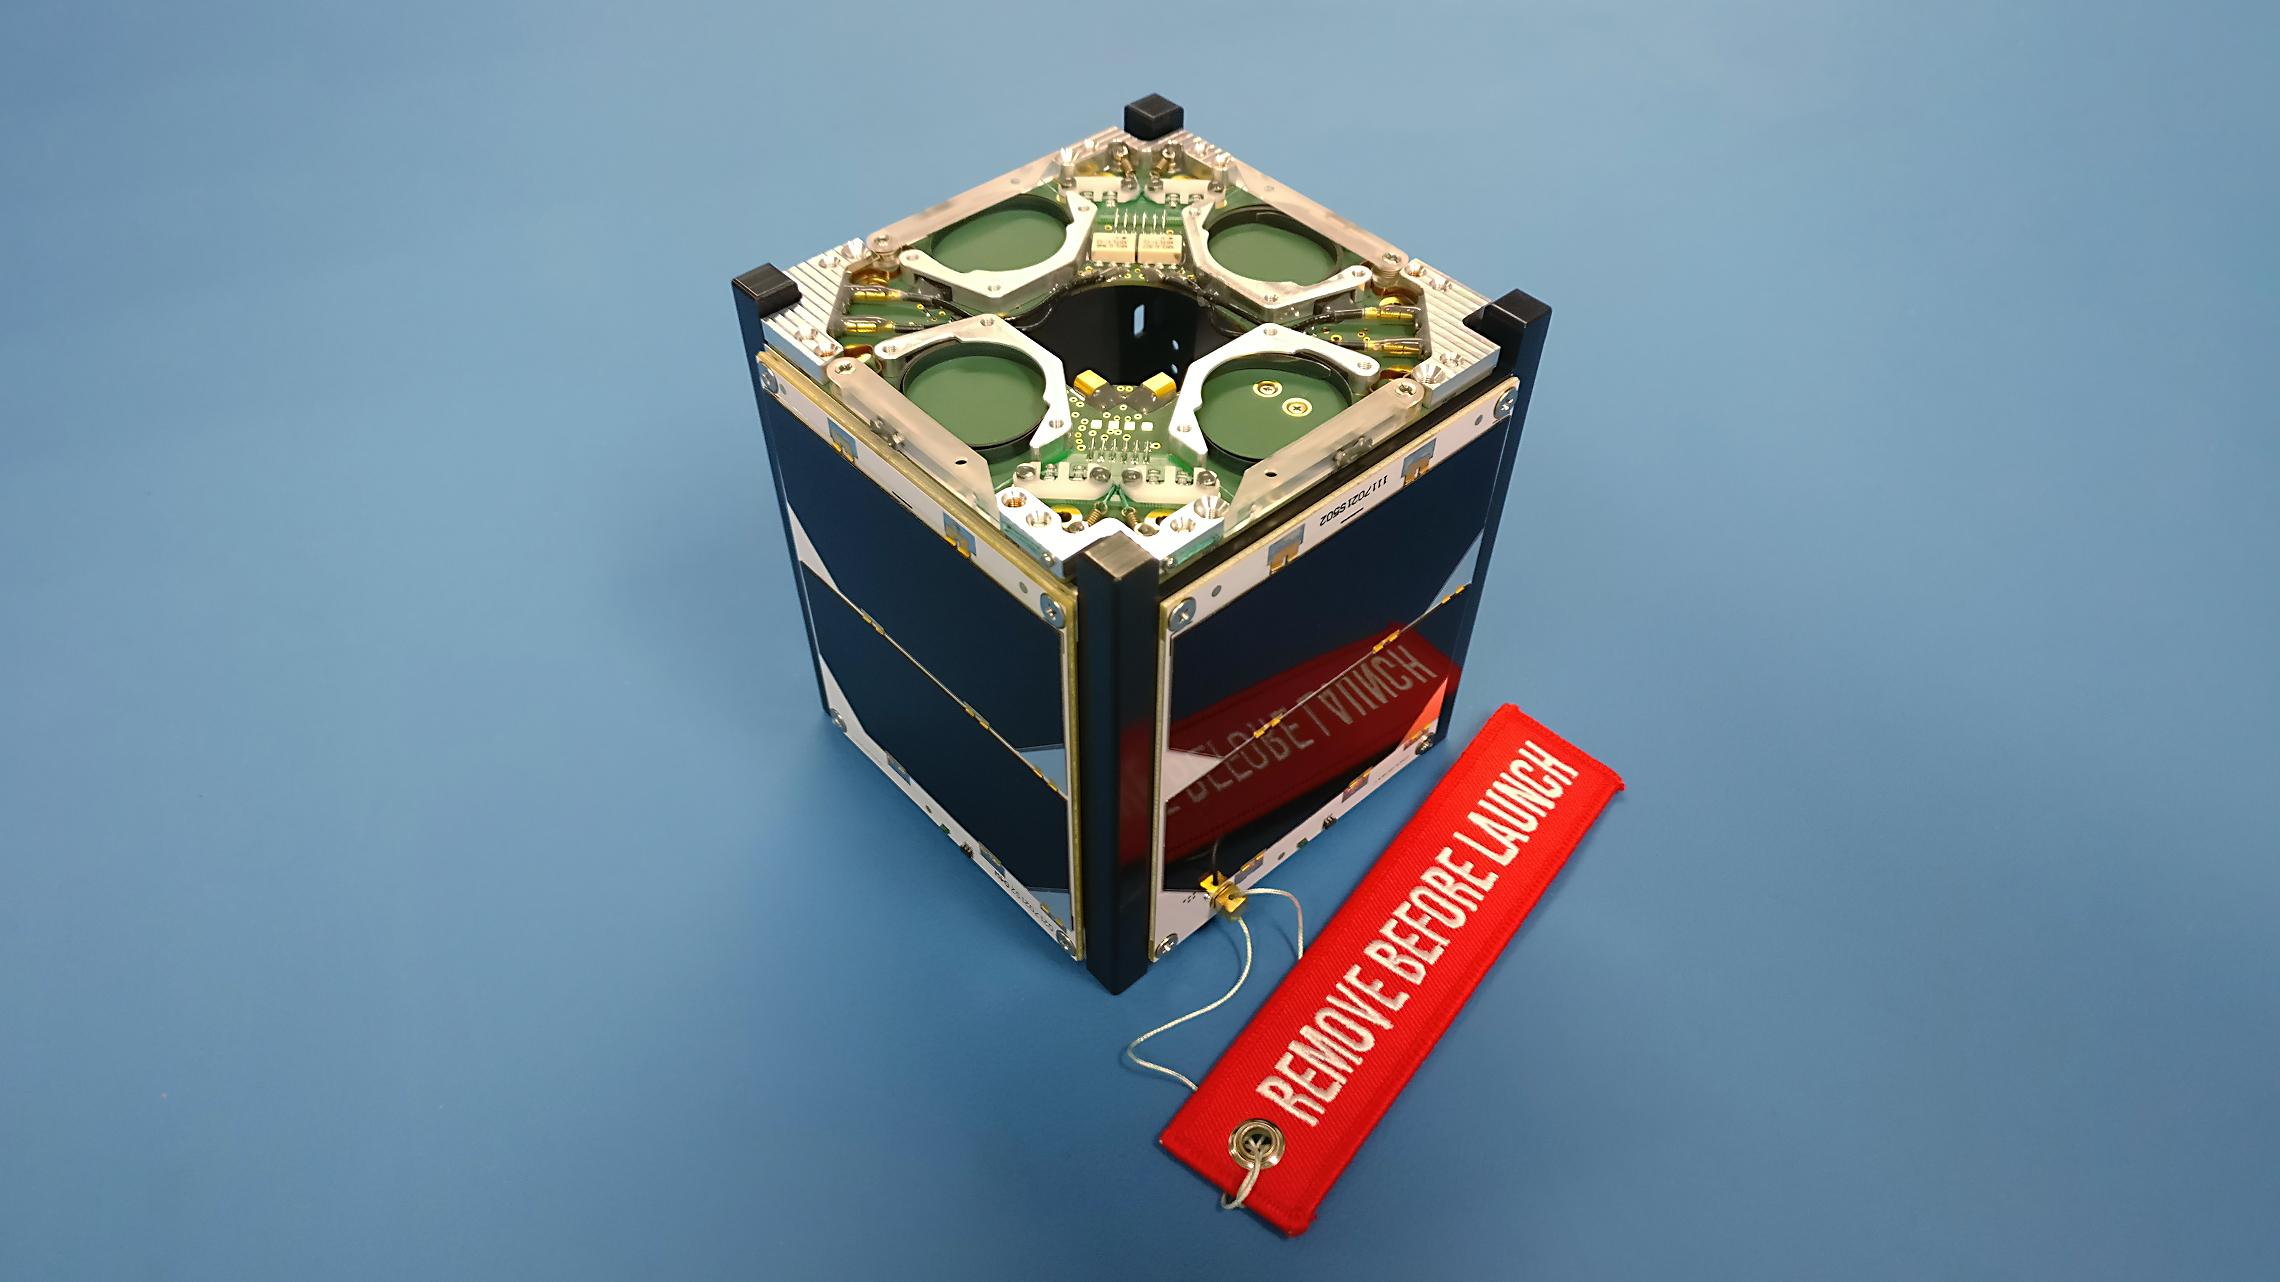
\includegraphics[width=0.95\textwidth]{images/istsat1.jpeg}
        \caption{Another independent caption.}
		\label{fig:four_in_row_4}
    \end{minipage}
\end{figure}

For more than 1 row of figures follow the example of Figure \ref{fig:five_images}.

\begin{figure}[!htb]
	\centering

    \begin{subfigure}[t]{0.3\textwidth}
        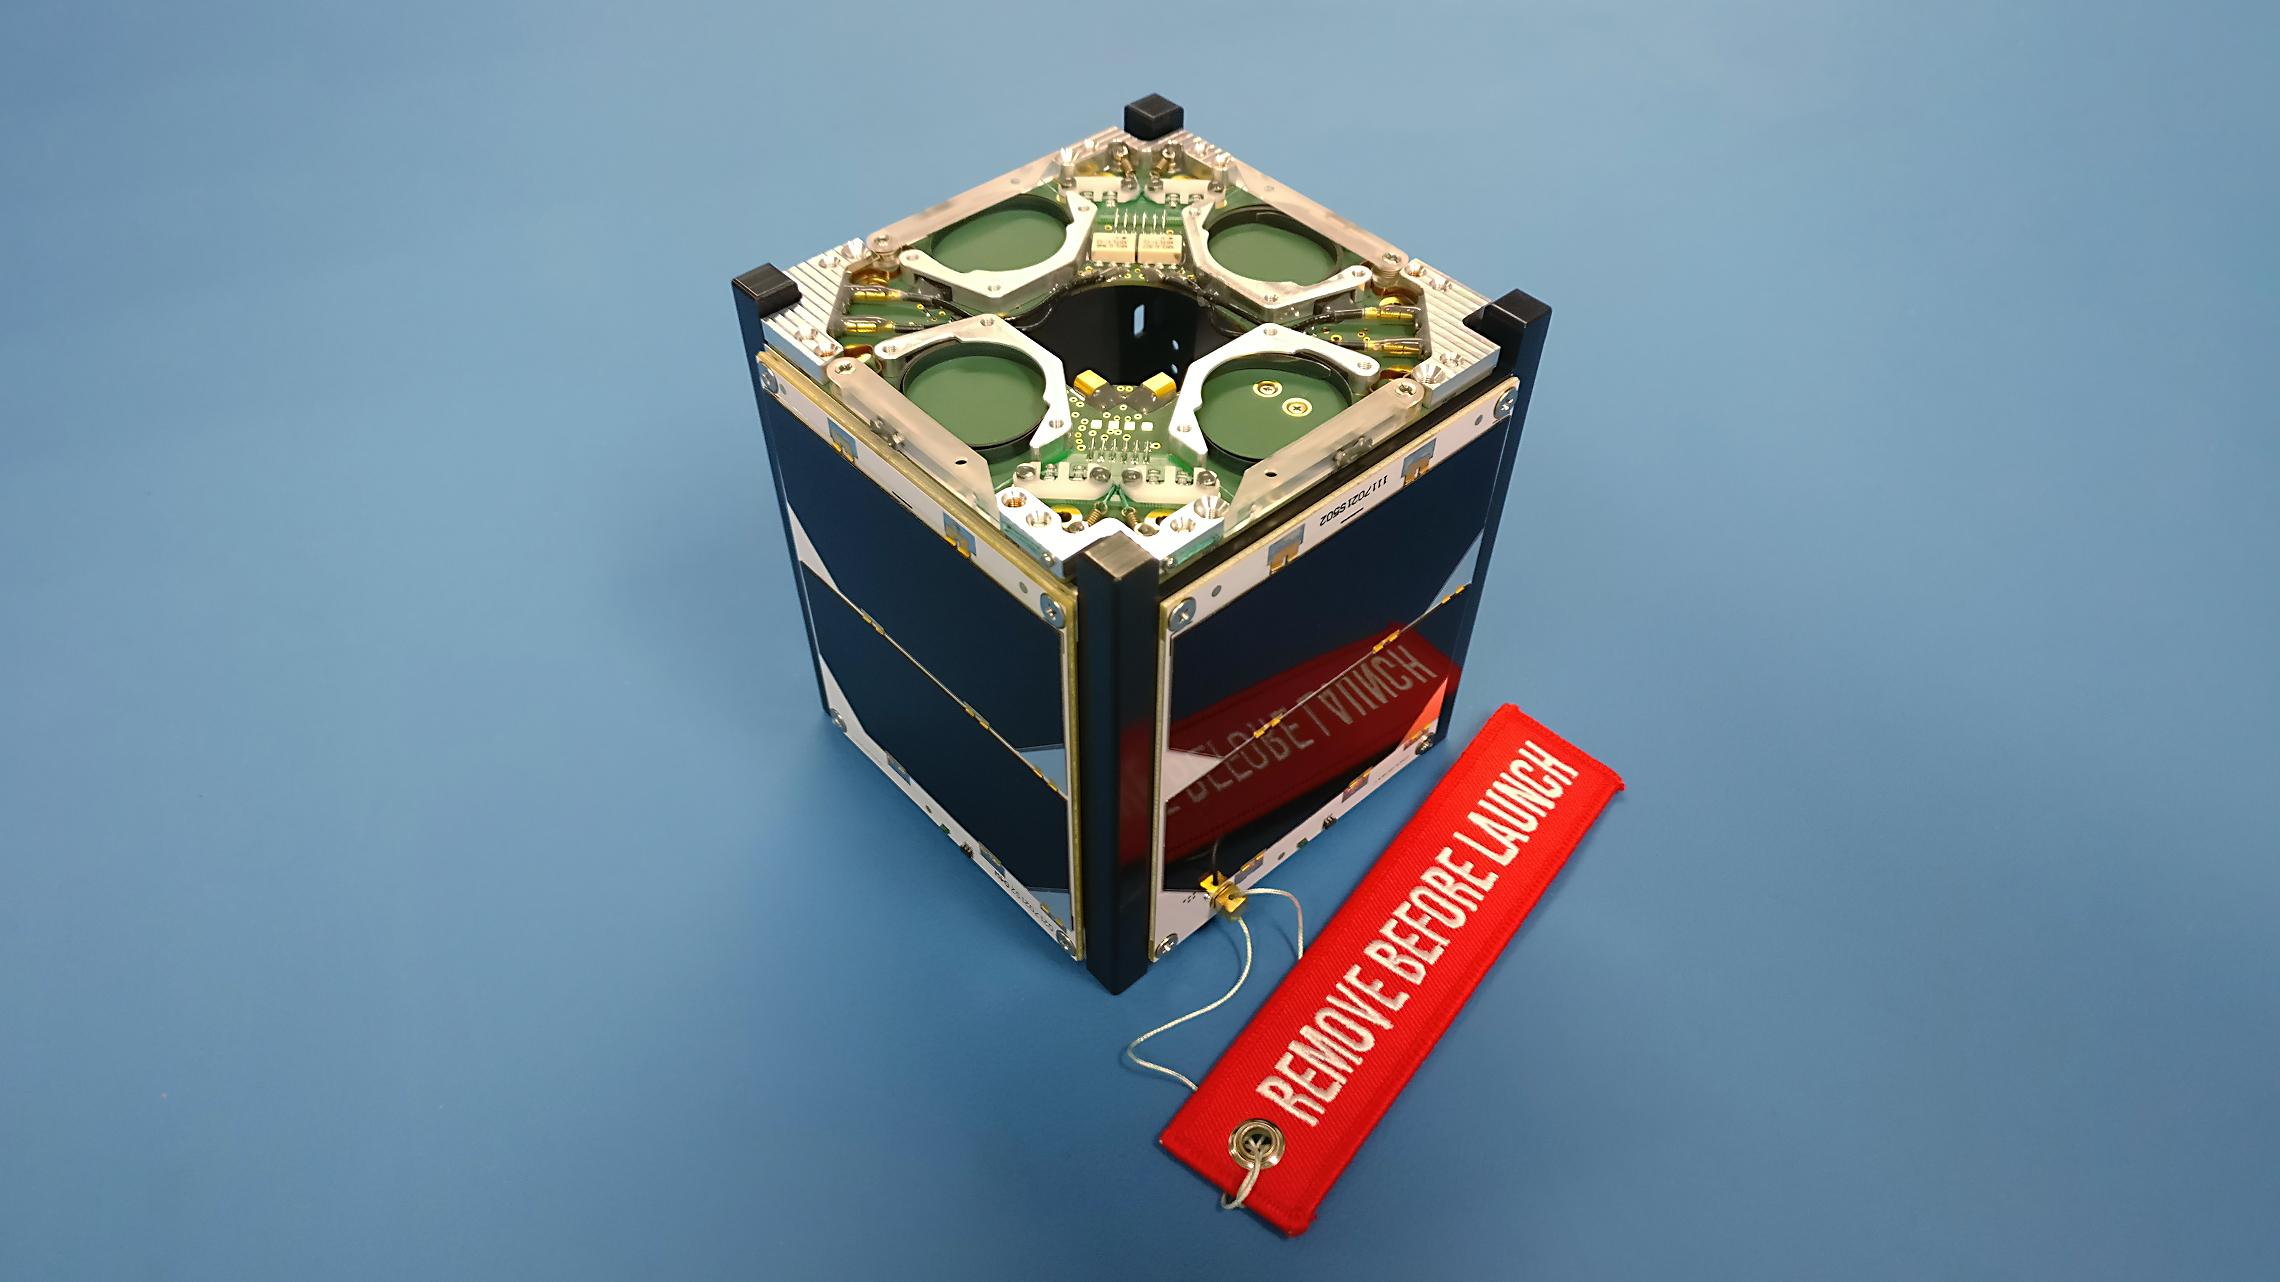
\includegraphics[width=\linewidth]{images/istsat1.jpeg}
		\caption{A caption.}
    \end{subfigure}
	\hfill
    \begin{subfigure}[t]{0.3\textwidth}
        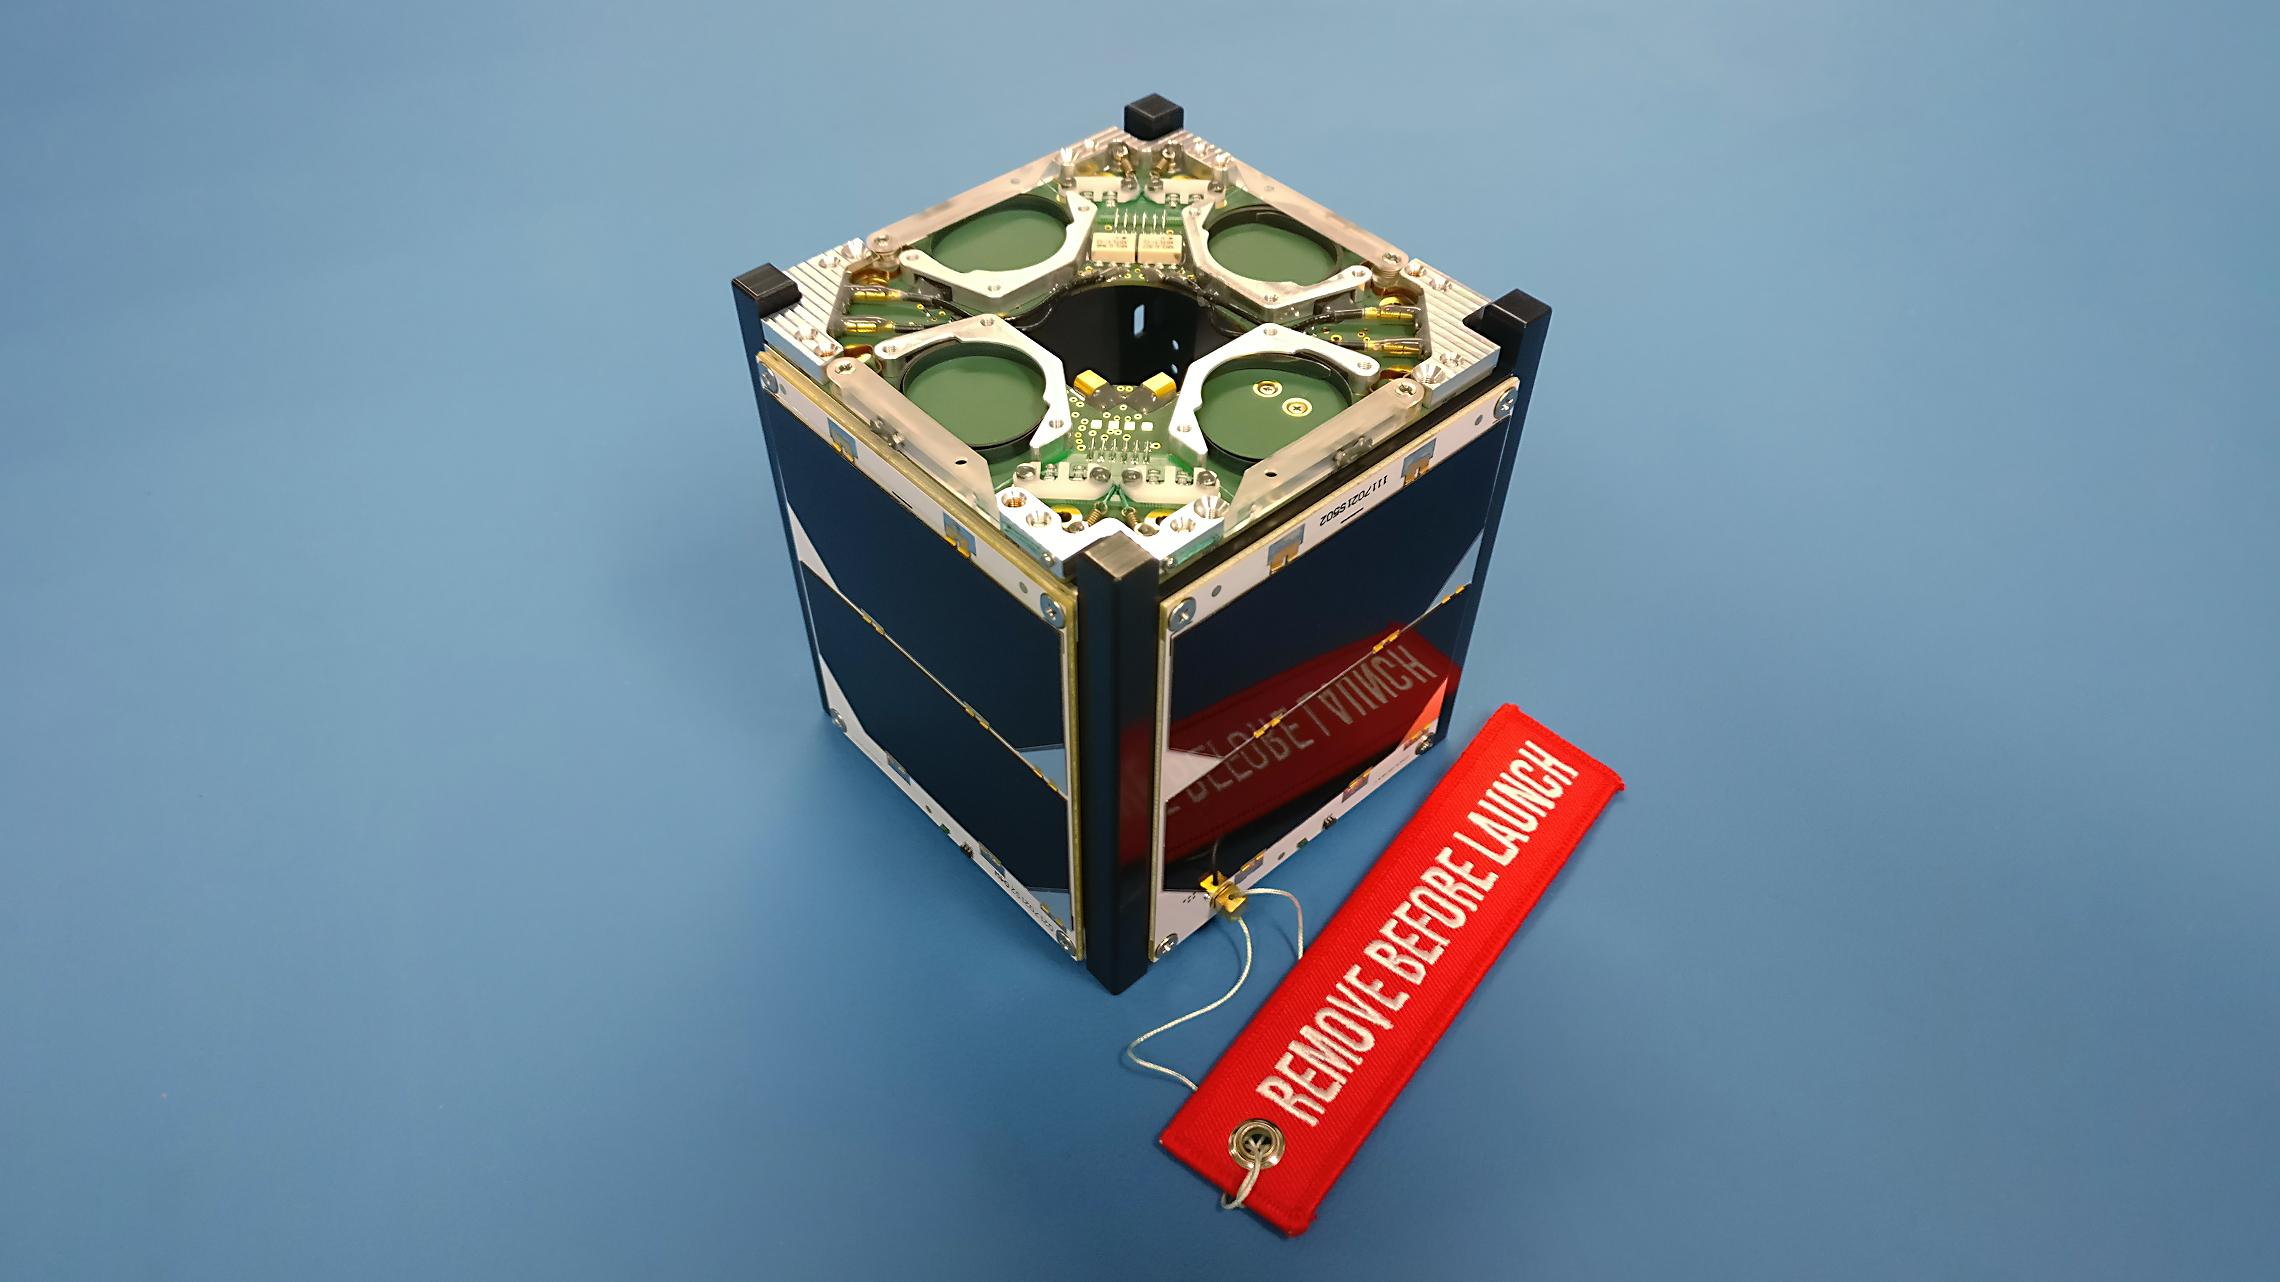
\includegraphics[width=\linewidth]{images/istsat1.jpeg}
		\caption{A caption.}
    \end{subfigure}
	\hfill
    \begin{subfigure}[t]{0.3\textwidth}
        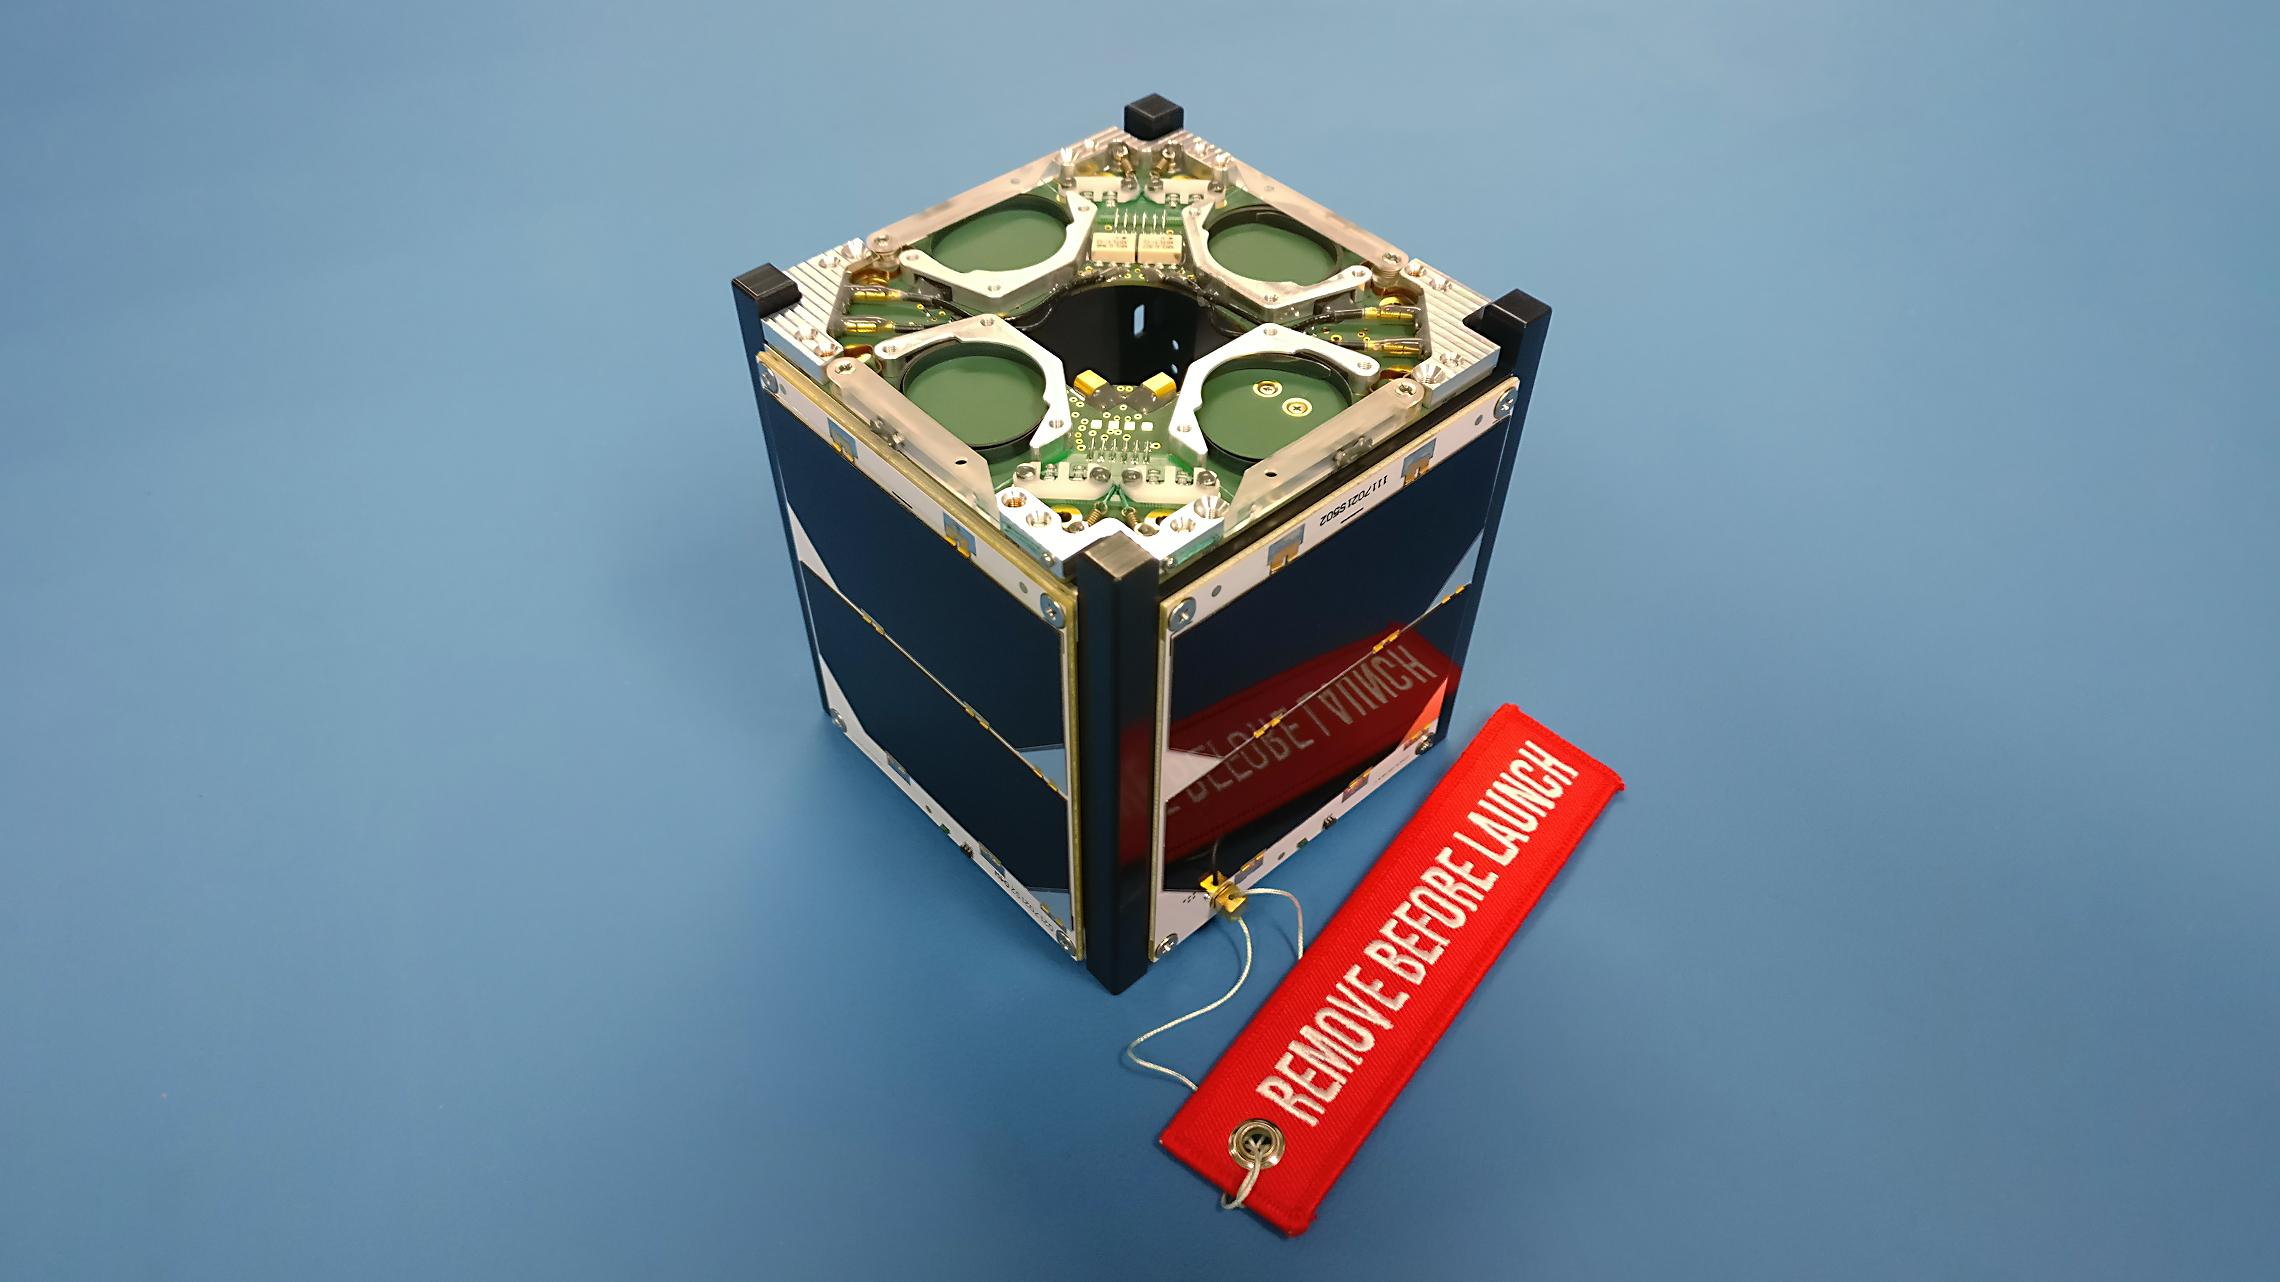
\includegraphics[width=\linewidth]{images/istsat1.jpeg}
		\caption{A caption.}
    \end{subfigure}

	\vspace{0.4cm}

    \begin{subfigure}[t]{0.3\textwidth}
        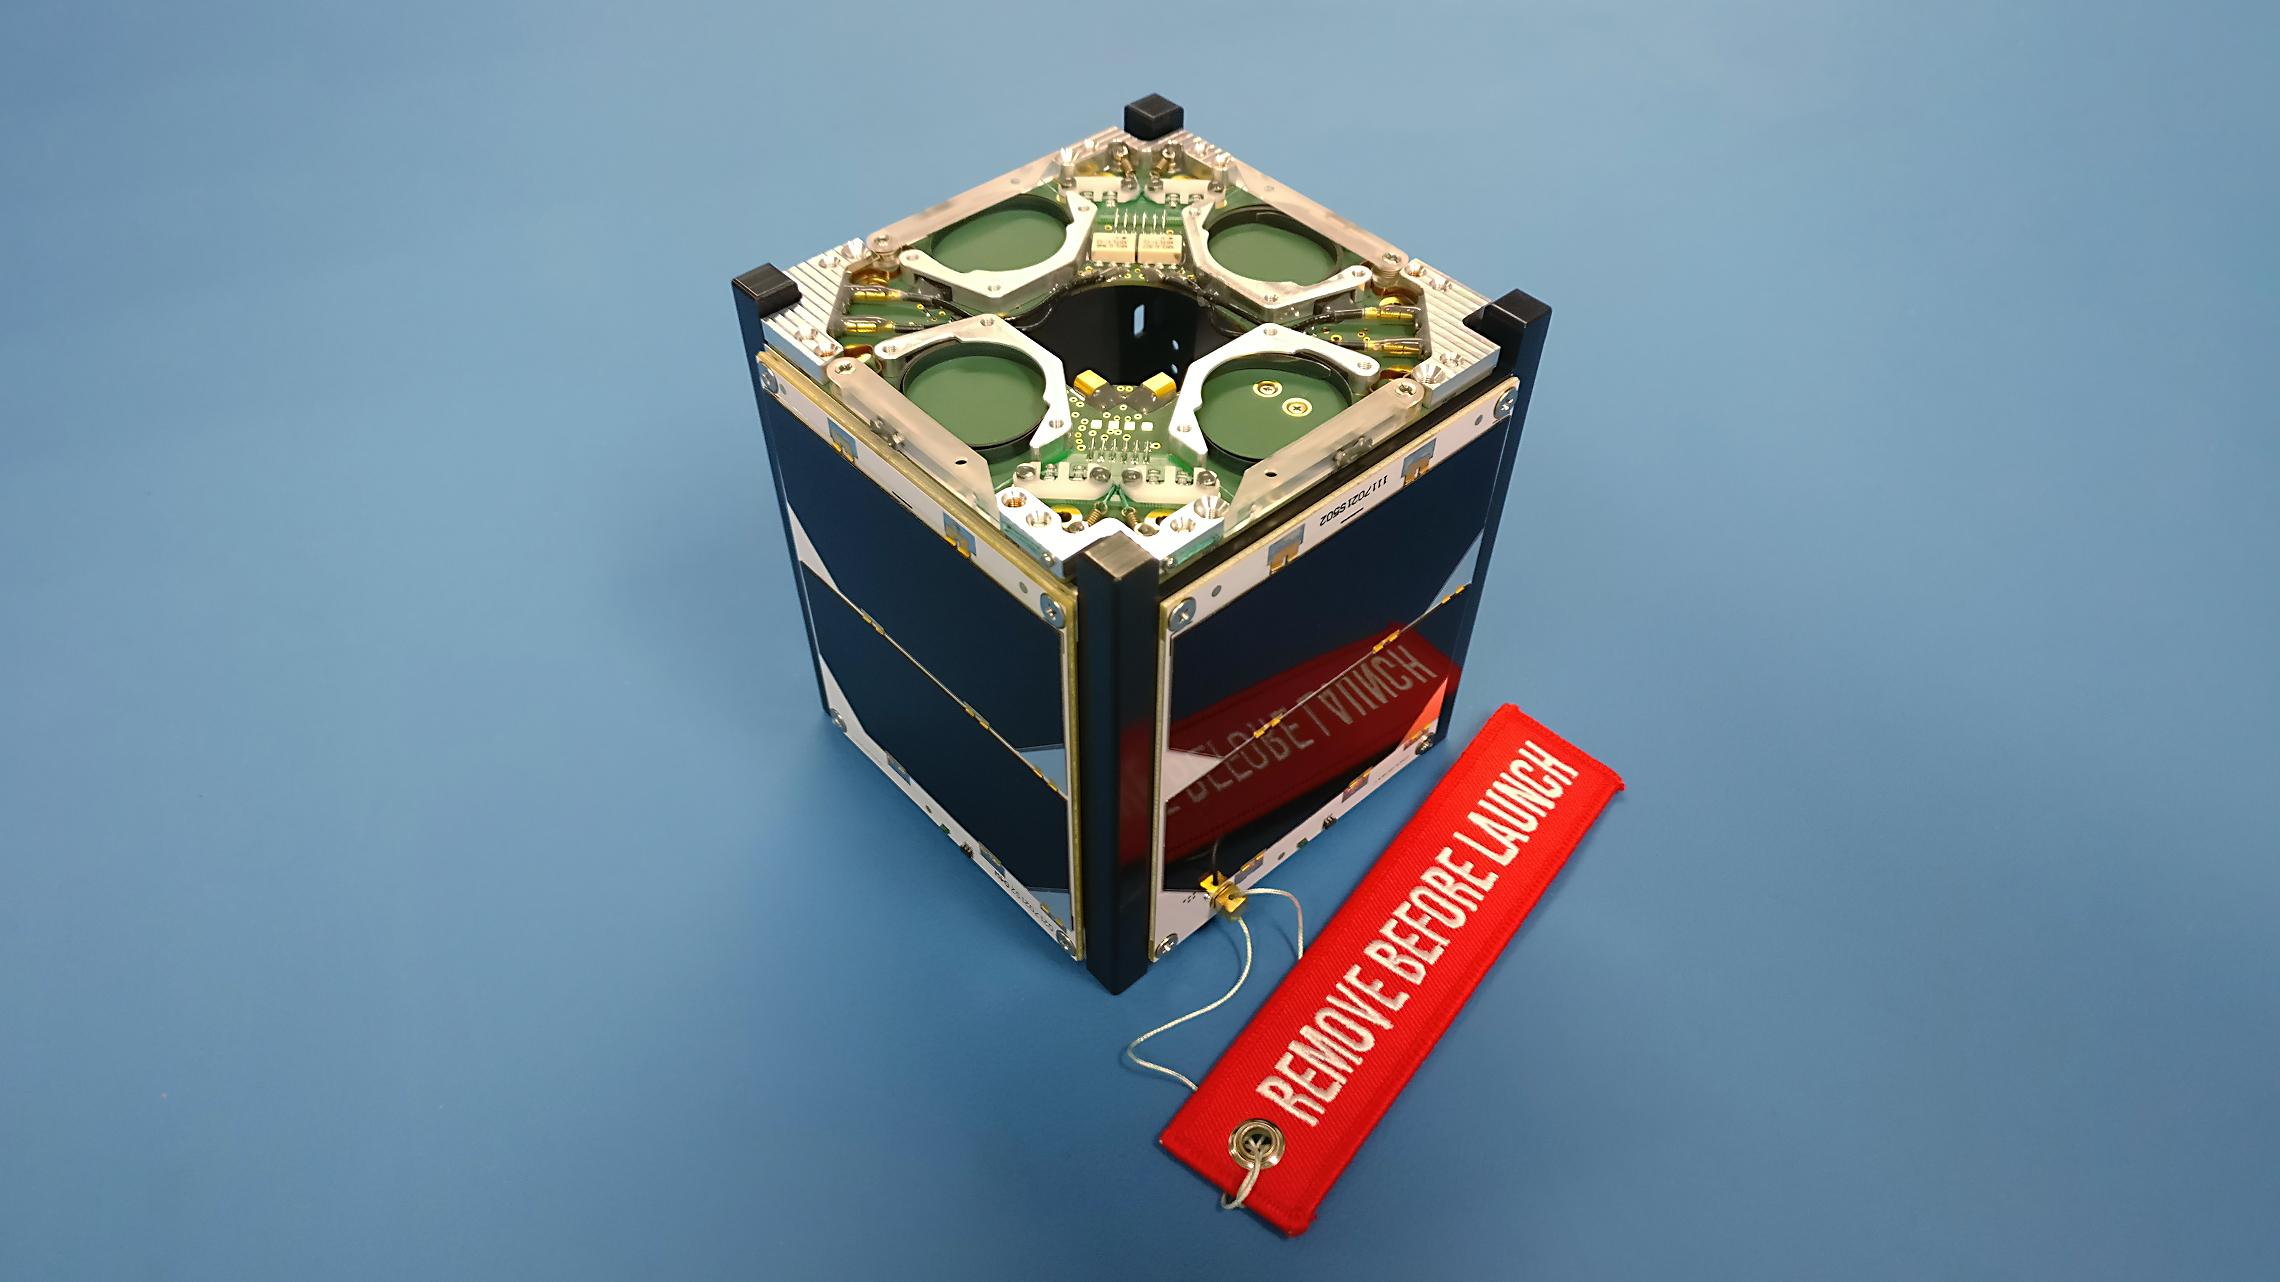
\includegraphics[width=\linewidth]{images/istsat1.jpeg}
		\caption{A caption.}
    \end{subfigure}
	\hspace{0.05\textwidth}
    \begin{subfigure}[t]{0.3\textwidth}
        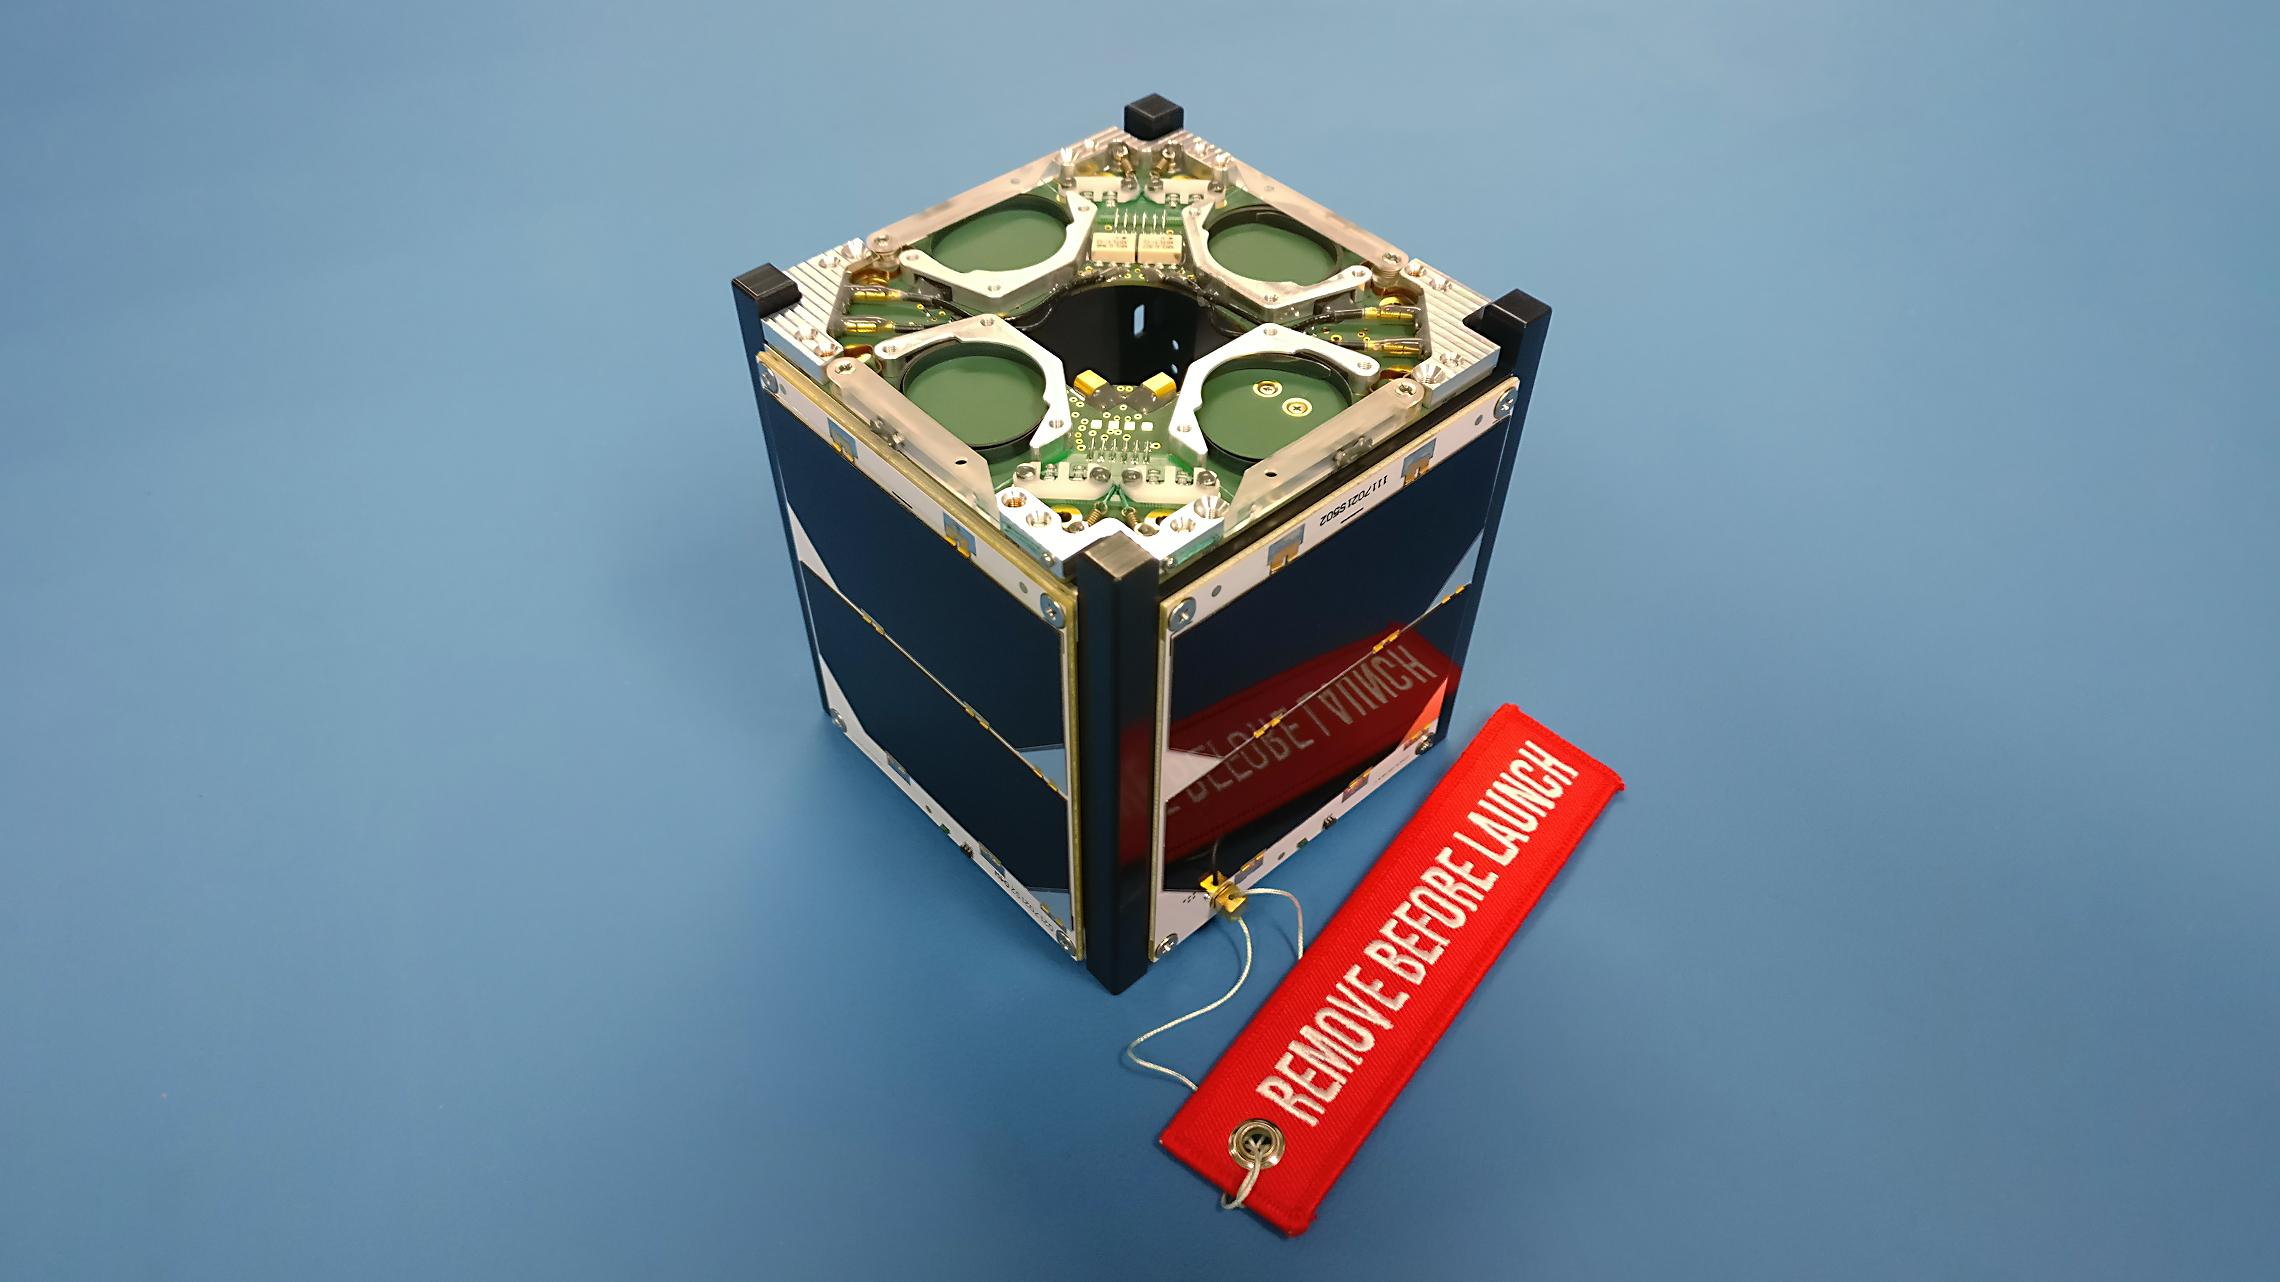
\includegraphics[width=\linewidth]{images/istsat1.jpeg}
		\caption{A caption.}
    \end{subfigure}

    \caption{This example is using the subfigure environment.}
	\label{fig:five_images}
\end{figure}